\documentclass[12pt,mscthesis]{usiinfthesis}

\usepackage{lipsum}
\usepackage{graphicx}
\usepackage{float}
\usepackage{cleveref}
\graphicspath{ {figures/} }

\usepackage{listings}
\usepackage[autostyle]{csquotes} 

\usepackage{subfig}

\lstdefinelanguage{algebra}
{morekeywords={import,sort,constructors,observers,transformers,axioms,if,
else,end},
sensitive=false,
morecomment=[l]{//s},
}



\title{Assessing Documents by Comprehension Effort } %compulsory
%\specialization{Dependable Distributed Systems}%optional
%\subtitle{Subtitle: Reinventing the World} %optional 
\author{Talal El Afchal} %compulsory
\begin{committee}
\advisor{Prof.}{Michele}{Lanza} %compulsory
\coadvisor{Prof.}{Gabriele}{Bavota}{} %optional
\coadvisor{Dr.}{Luca}{Ponzanelli}{}

\end{committee}
\Day{1} %compulsory
\Month{September} %compulsory
\Year{2017} %compulsory, put only the year
\place{Lugano} %compulsory

\dedication{To my beloved} %optional
\openepigraph{Your living is determined not so much by what life brings to you as by the attitude you bring to life; not so much by what happens to you as by the way your mind looks at what happens}{Gubran Khalil Gubran} %optional

%\makeindex %optional, also comment out \theindex at the end

\begin{document}

\maketitle %generates the titlepage, this is FIXED

\frontmatter %generates the frontmatter, this is FIXED

\begin{abstract}
Recommender systems for software engineering have become increasingly popular in recent years. These systems combine several methodologies to provide suggestions that meet the developer's needs. Recommender systems collect data from online resources as blogs, forums, Q\&A websites, and suggest documents or piece of code that are most likely helpful to the developers. However, these systems are not taking into consideration an important aspect as the comprehension effort, which may vary depending on the document familiarity and readability. Usually developers are more interested in documents which they are familiar with. By calculating the comprehension effort, the recommender system can complement the rank and suggest the most comprehensive and appropriate ones to the developer. In this work, we present our approach to calculating the comprehension effort, by creating a language model able to capture a document familiarity, that we combine with the document readability. 
\end{abstract}

\begin{acknowledgements}
\end{acknowledgements}

\tableofcontents 
\listoffigures %optional
\listoftables %optional

\mainmatter

\chapter{Introduction}

	\section{Context}
	The complexity of software systems is increasing and new technologies are introduced constantly \cite{Lehman:1985:PEP:7261}. Software developers often have to work with new technologies which they are not familiar with, and as increasingly more comes out, the amount of information that they need to know will increase. For example, Android\footnote{\url{https://www.android.com}} was introduced 10 years ago in 2007, and in 2008 the first version was released, and nowadays, there are 8 versions of Android. 
	

	When Android started to become popular, developers had to learn this technology and stay updated with each new release.
	They had to search how activities work in Android, and how to use several APIs to implement different tasks assigned to them.
	However, the process of searching the right piece of information as a tutorial or a documentation is time-consuming and requires considerable effort.
	For example, if an Android developer needs to use a new Android API that is completely new to her. She will search for web artifacts such as forums, blogs, questions and answers (Q\&A) websites, and API documentation \cite{Sim:2011:WSE:2063239.2063243}.


	The amount of resources is vast, a popular Q\&A websites as Stack Overflow contains a million of questions tagged as Android\footnote{\url{https://stackoverflow.com/questions/tagged/android}}. Github, one of the most popular version control system where developers can store their projects, hosts more than 500 thousand Android repositories\footnote{\url{https://github.com/search?utf8=✓&q=android&type=}}, with millions of lines of code which can be an important resource.


	A tool helping developers to gather information among the available resources would ideally improve the search process, that would result in time saved for the developers.
	Similar tools to suggest items of interest already exists outside the context of software engineering, for example Amazon\footnote{\url{https://www.amazon.com}}, Ebay\footnote{\url{https://www.ebay.com}} and Netflix\footnote{\url{https://www.netflix.com/ch-en/}}, employ recommender systems to suggest their products.


	What is a recommender system? The proposed definition by the organizers of the ACM International Conference on Recommender Systems \footnote{\url{https://recsys.acm.org/recsys09}} is: \\

	  \blockquote{\textit{``Recommendation systems are software applications that aim to support users in their decision-making while interacting with large information spaces. They recommend items of interest to users based on preferences they have expressed, either explicitly or implicitly. The ever-expanding volume and increasing complexity of information [...] has therefore made such systems essential tools for users in a variety of information seeking [...] activities. Recommendation systems help overcome the information overload problem by exposing users to the most interesting items, and by offering novelty, surprise, and relevance.''}}

	  In the context of software engineering, developers need other items useful to their scope as tutorials, code snippet and libraries. Recommender system targeting similar items are known as recommender systems for software engineering (RSSE). According to \citet{RecommendationSystemsforSoftwareEngineering} 
	\emph{``An RSSE is a software application that provides information items estimated to be valuable for a software engineering task in a given context''}.
	

	There is a vast number of proposed RSSEs, some of them suggest relevant project artifacts or code examples \cite{Holmes:2005:USC:1062455.1062491} \cite{Cubranic:2003:HRP:776816.776866} \cite{Zimmermann:2004:MVH:998675.999460}. Other focused on suggesting relevant code samples, documents and discussions from the web resources \cite{Rahman:2015:RRS:2886444.2886471} \cite{Sawadsky:2011:FTC:1984708.1984722} \cite{Stylos:2006:MWT:1174509.1174678} \cite{10.1109/VLHCC.2012.6344497}. But none of them has considered the required effort to comprehend the suggested documents.


	Searching for documentation and tutorials is a crucial step in learning a new technology. Developers can find a bunch of online resources as blogs, forums, Q\&A websites, but the real challenge is to find the most suitable one for their needs. \citet{Singer-1997} reported in 1997 that the most frequent developer activity was code search, and \citet{Sadowski:2015} did a case study on how developers at Google search for code. They figured out that developers are generally seeking answers to questions about how to use an API, what code does, why something is failing, or where the code is located. The interesting point in this study was the fact that most searches focus on code that is familiar, or somewhat familiar to the developers.
	Therefore, we believe that RSSE has to take into consideration the familiarity of a document when they suggest it to the developer. 

	
	Understanding a document is a cognitive process, and it depends on the human brain intelligence, yet if we are familiar with a subject, we will likely comprehend it with less effort. For example, a computer engineer might comprehend a document explaining how to implement a sorting algorithm, with much less effort compared to a document that explains a constitutional law, and the reason is not that the algorithm is simple, but because a computer engineer is more familiar with sorting algorithms than law.
	

	In this thesis, we try to evaluate similar situations. For example, given two documents that have approximately the same subject, how can we decide which one is easier to comprehend? To answer this question we need to introduce two concepts:
	\begin{itemize}
	\item \textbf{Familiarity}: how much are developers familiar with the document content?
	\item \textbf{Readability}: how difficult is it to read a given document?
	\end{itemize}
	The familiarity and readability metrics are important for us, since the comprehension effort can be derived from the document familiarity and readability.\\
	For example, if we want to use a tool that gives us a score to indicate which document requires less effort to be comprehended, where a higher score indicates a high effort, and we have two documents where, in the first one we have an Android task implemented in Android 7.1 and in the other document we have the same task implemented in Android 4.0, and the developer is familiar with Android 7.1.
	We expect that the first document must have a lower score since logically it requires less effort to be comprehended by developers who are more familiar with Android 7.1.
	What if both documents have the same task, and both tasks are implemented with the Android 7.1 ? Which one will have a lower score? 
	In this case, the document readability has a big impact on the comprehension effort: The developer would likely prefer to read the document with the best readability.\\
	
	\section{Objective and Results}
	Our main goal in this thesis is to assess documents by their comprehension effort, which can be leveraged by RSSE to improve their suggestions.
	To calculate the comprehension effort we need to find a way to compute the familiarity, and we need to evaluate our approach to understand if it effectively works.
	To evaluate our approach we run two studies:\\

	 In the first study we evaluate our familiarity approach. We select a big set of Android documents, which represents the hypothetical developer knowledge, where a document can be a mix of code and natural language. Then we create a \emph{ Language Model} \cite{Hindle:2012:NS:2337223.2337322} and we train it with these documents (training set). In this way, we are able to simulate the context of a developer who is familiar with Android. Once we trained the language model, we evaluate the familiarity of a given set of documents (testing set) that contains Android documents and other documents that are not related to Android.


	 The language model was able to evaluate the Android documents within the testing set as thousand times more familiar than the rest. 
	 In this experiment, the language model approach satisfied our expectation in capturing the document familiarity.\\

	 In the second study we evaluate our approach in assessing documents by the comprehension effort. In this study we ask developers to read a set of tutorials, and then we give them a set of documents, where some documents are related to the tutorials and some are not, and we ask the developers to score the documents by the comprehension effort. and we compare their scores with our precomputed scores. The evaluation results suggest that our approach is promising in estimating the comprehension effort of developers. 


	\section{Structure of the Thesis}
	This thesis consists of seven chapters: 
	\begin{enumerate}
	
		\item \textbf{Introduction}: In this chapter we introduce the thesis work.
		\item \textbf{State of the Art}: This chapter describes the existing related work as code search engines, and recommender systems.
		\item \textbf{Approach}: This chapter describes our approach to calculate the comprehension effort.
		\item \textbf{Study design}: This chapter discusses the research question, the data extraction process, the analysis method, and the replication package.
		\item \textbf{Result}: This chapter shows the results and their implication.
		\item \textbf{Threat to Validity}: This chapter describes the possible threats that could affect the results validity.
		\item \textbf{Conclusion}: This chapter summarizes our work, and presents some ideas for a possible future work, and concludes the thesis.
	\end{enumerate}
\chapter{State of the Art}
	In this chapter, we present the existing related work to the comprehension effort, and discuss other related tools, as code search engines and recommender systems.
\section{Program Comprehension}
	There are several studies on program comprehension and in this section we mention few of them, that are related to the thesis work. \\


	\citet{Corbi:1989:PUC:97118.97124} did a research on tools which could help developers in two key areas: static analysis (reading the code) and dynamic analysis (running the code). In this paper Corbi describes how program understanding relates to software renewal, and he indicates that more than half of the time is spent in understanding the system. Corbi concludes the paper by mentioning that developer training and tools should show or assist the developer in combining  different kinds of information in ways which can support his or her understanding of the system being investigated, and they should not favor or force the use of only one way of gathering information about programs.
	This paper motivates us to investigate and develop a novel technique to calculate the comprehension effort.
	\newpage

	Another related work is by \citet{Kushwaha:2006:ICI:1163514.1163533}  who claim that the required effort to understand a software depends on the difficulty in understanding the information, where the information is related to the number of operators and identifiers. They count the number of operators and identifiers per line of code and they multiply it by an associated weight of the identifier name ( 1 if the identifier name belongs to the problem domain, and 4 is the identifier name is selected arbitrarily). 


	They performed an experiment on 60 students, where 5 sample programs were given. One set of programs had meaningful identifier names related to the problem domain and the other used arbitrarily selected identifier name. They measured the required time to comprehend the program.


	The result showed that programs with arbitrarily selected identifier names required about 4 times the time needed to comprehend the programs compared to programs with meaningful identifiers.\\


	\citet{Scalabrino} presented a metric able to assess the understandability of a given code snippet . In their work they consider three types of metrics:
	\begin{enumerate}
		\item \textbf{Code-related metrics} are metrics related to the code, (e.g., cyclomatic complexity, LOC, the number of identifiers, line length).
		\item \textbf{Documentation-related metrics} capture the quality of the internal documentation of a snippet (e.g, comments readability, and identifiers consistency). 
		\item \textbf{Developer-related metrics} measure the programming experience of the developer in years, in any programming language.
	\end{enumerate}
	They analyze whether code-related, documentation-related, and developer- related metrics can be used to assess the understandability level of a snippet  code. The authors asked
	46 developers to carefully read and to fully understand eight code snippets. Participants could, in any moment select the option \textit{I understood the snippet} or \textit{I cannot understand the snippet}, and the time was monitored.
	Once the participant choosed \textit{I understood the snippet} option, the authors asked questions about the code snippet to verify the actual level of understanding.

	After an extensive statistical analysis \citet{Scalabrino} couldn't find a significant correlation between the considered metrics and the understandability of code snippets.
	They assumed that the code complexity has a big influence on the developer' ability to understand the code, but they couldn't demonstrate it with a strong empirical evidence.They also mentioned that the code readability can have a direct impact on the understandability of the code.\\ As mentioned in the previous chapter, in this thesis we take in consideration the code readability to calculate the comprehension effort.\\

	\citet{Buse2010} introduced a code readability metric, and they investigate its relation to software quality. A part of their work was to run an experiment which compared readability of the code to the cyclomatic complexity, and they were able to show that code readability is significantly independent of the traditional code complexity.


	In this experiment, 120 developers were asked to individually score a sequence of 100 code snippets, based on their personal estimation of readability. From the result, they determined which code features were predictive of readability, and they construct a readability model. They also tested the model performance on ten different classifiers, and on average the model classified correctly between 75\% and 80\% of the snippets.They found that factors like \textit{average line length} and, \textit{average number of identifiers per line} are very important to readability.In this thesis we use \citet{Buse2010} approach to calculating code readability.

	\section{Semantic code search and code search engines }

	\citet{Reiss:2009:SCS:1555001.1555040} presented a tool that generates specific functions or classes from the open source repositories, where these classes meet user's specifications. This tool uses the user's input, as keywords and other constraints, and suggests codes that meet the user's needs.


	The tool takes a set of candidate solutions, and it transforms it into a more appropriate set. Both static and dynamic specifications can be used. This tool main goal is to satisfy the user's constraint, but it does not take into consideration the user's experience and the comprehension effort.\\
	

	\citet{Thummalapenta:2007:PPA:1321631.1321663} presented \emph{PARSEWeb} a tool similar to \citet{Reiss:2009:SCS:1555001.1555040}, where they collect code from public sources and search engine suggest it to the developer based on their input query.\\ In the query, the developers have to specify the \textit{source object type} and the \textit{destination object type}.  For example, programmers know what type of object that they need to instantiate like \emph{QueueConnectionFactory} (Source), but do not know how to write code to get that object from a known object type like \emph{QueueSender} (Destination). Therefore, the proposed problem can be translated to a query of the form \emph{QueueConnectionFactory} \rightarrow \emph{QueueSender}.

	\citet{McMillan:2011:FRF:1985793.1986032} created an application search system called \textit{Exemplar}, which reduce the mismatch between the high-level intent reflected in the descriptions of software and low-level implementation details.

	 \textit{Exemplar} differs from the traditional search engine that matches the keywords, by matching keywords with the descriptions of the various API calls in help documents.
	\textit{Exemplar} has three components of Ranking: 
	\begin{enumerate}
		\item \textbf{WOS} a component that computes a score based on word occurrences in project descriptions
		\item \textbf{RAS} a component that computes a score based on the relevant API calls
		\item \textbf{DCS} a score based on data-flow connections between calls
	\end{enumerate}
	In this paper \citet{McMillan:2011:FRF:1985793.1986032} concludes by mentioning that the performance of search engines can be improved if those engines consider the API calls that the software uses.\\

	
	\citet{Bajracharya2012} conducted an exploratory analysis of the usage log of Koders, the first commercially available Internet-Scale code search engine, and their goal is to answer the following three questions:\\
	\begin{enumerate}
	\item \textbf{Usage}: What kind of usage behavior can we see in Koders?
	\item \textbf{Search Topics}: What are the users searching for?
	\item \textbf{Query Forms}: How are users expressing their information need in their queries?
	\end{enumerate}
	They start analyzing the usage logs, and they get the following results: 
	\begin{itemize}
	\item Most of the users did not use Koders again after using it for a day
	\item Sessions are short (a series of activities by a single user within a small duration of time constitutes a session )
	\item More than half of the sessions had no downloads
	\item There are few sessions with no search activities
	\item Queries are very short
	\item Terms in queries are quite diverse
	\item Code queries are the mostl used types of queries
	\item Code queries lead to the most of the downloads
	\end{itemize}
	they conclude the analysis by mentioning that usage behavior is similar between Koders and search on the Web, and the majority of the users don't refine their existing queries.\\

	The approaches described so far, do not take into consideration any readability or familiarity metrics. We believe that our comprehension effort metric can be integrated in in these search engines as complementary information to help the user in choosing the must relevant document.
	
	\section{Recommender Systems for Software Engineering}

	\citet{Cubranic:2003:HRP:776816.776866} built Hipikat, a tool that helps newcomer to become productive more quickly, by recommending existing artifacts from the development that are relevant to a task that the newcomer is trying to perform. Hipikat infers links between the artifacts that may have been apparent at one time to members of the development team but that were not recorded, and then Hipikat uses this links to suggest possibly relevant parts of the group memory given information about a task a newcomer is trying to perform.\\
	The authors performed two qualitative studies, where they show that Hipikat approach helped newcomers to perform a task effectively on an unfamiliar system.\\


	\citet{Holmes:2005:USC:1062455.1062491}  built the Strathcona tool, a plug-in for the Eclipse integrated development environment (IDE), the tool extracts the structural context of the code on which a developer is working, and selects from an example repositories a set of relevant code examples to be returned using a set of structural matching heuristics.


	To understand if the structural matching heuristics can return examples that a developer finds useful, \citet{Holmes:2005:USC:1062455.1062491} performed a case study in which they asked two developers to complete four programming tasks, where Subject 1 had less than one month of Eclipse plug-in programming experience but more than eight years of Java experience. Subject 2 had over six months of Eclipse plug-in programming experience but only eighteen months of experience with Java, and neither subject knew how to implement any of the assigned tasks.
	Subject 1 completed all four tasks successfully, finding relevant examples in all cases for which appropriate examples were returned; Subject 2 completed three out of four tasks, finding relevant examples in two of the three cases. These results show that Strathcona can suggest relevant examples to developers.\\

	\citet{Ponz2014b} built the Prompter tool, a plug-in for the Eclipse integrated development environment (IDE), that retrieves and recommends, with push notifications, relevant Stack Overflow discussions to the developer. Prompter analyzes the code context in the IDE and searches for Stack Overflow discussions, evaluates their relevance by taking into consideration \emph{code aspects}, \emph{conceptual aspects}, \emph{community aspects}.


	The authors performed a study to evaluate to what extent the use of Prompter can be useful to developers during a development or maintenance task. In the study they selected 12 participants that have at least 3 years of experience in programming, with a maximum of 12. The authors asked the participants to perform one maintenance task and one development task, and then the authors asked them if they have used the suggestions by Prompter. Three participants answered \emph{absolutely yes}, eight \emph{more yes than no}, and two \emph{more no than yes}.


	Ponzanelli et al. concluded their work by mentioning that Prompter ranking model resulted to be effective in identifying the right discussions given a code snippet to analyze.\\


	
	In a following paper \citet{Ponz2017a} created LIBRA, a holistic recommender system that supports developers in their information search in the web browser. The developers are tracked during their activities in the IDE and in the web browser, which allows Libra to collect information as web search results, perused pages, and code written and modified by the developer. LIBRA uses this information to model a knowledge context of the developer and, constructs a holistic meta-information model of their contents.
	

	LIBRA is based on three important metrics :
	
	\begin{itemize}
	\item \textbf{Context Complementarity} measures the information intake provided by a resource in the current context of the developer. A low context complementarity indicates that the resource information is already a part of the context. In other words, the resource and the context are too similar, and the amount of new information that the developer can retrieve is low.
	
	\item \textbf{Result Prominence} identifies prominent results among the search engine result set. When a query matches a result, it doesn't tell us so much about the result relevance. If a result overlaps with many other results, it would be more prominent, since probably it provides diversified information in its contents.
	
	\item \textbf{Information Quantity} sums up the number of ``elements'' identified by LIBRA's meta-information system. This metric is important to distinguish which resource has more information giving two resources with a similar number of characters. If the first resource has only text and the second one has text and code, obviously the second resource contains a higher information quantity.
	\end{itemize}
	16 third year CS Bachelor students were asked to evaluate LIBRA in terms of \textit{its ability in correctly assessing for each query search result its prominence and complementarity with respect to the context, and usefulness to developers during a development or maintenance task.}\\
	The study results indicated that both prominence and complementarity indicators reflect developers’ perception of such measures, and are considered as useful indicators. Moreover, students  achieved a significantly better task completeness with LIBRA.\\

	The work that has been done in this thesis can be integrated with RSSE as LIBRA, where the comprehension effort metric can be added to the other three metrics used by LIBRA to provide developers with the most relevant documents.


\chapter{Approach}
	The volume of online resources is increasing, we can find millions of documents related to one search query. How can we suggest the most suitable one to developers? Several elements might determine which documents contain valuable information, and one of these elements is the comprehension effort. Code search has been a part of software development for decades, \citet{Singer-1997} reported in 1997 that the most frequent developer activity was code search, and most searches focus on code that is familiar to the developer \cite{Sadowski:2015}. Certainly, developers prefer to search for documents they are familiar with since they require less effort to be comprehended. We believe that the comprehension effort is strictly related to the document familiarity and readability.
     
    In the literature there are several metrics that estimate the readability of a given text, (e.g., Flesch$-$Kincaid \cite{Kincaid}, Dale$-$Chall \cite{Dale-Chall}), and other metrics that estimate code readability \cite{Buse:2010:LMC:1850489.1850615}. In this thesis, we introduce for the first time a new approach where we combine text readability, code readability and document familiarity, to estimate comprehension effort.\\

	
	
	\begin{figure}[H]
	\centering
	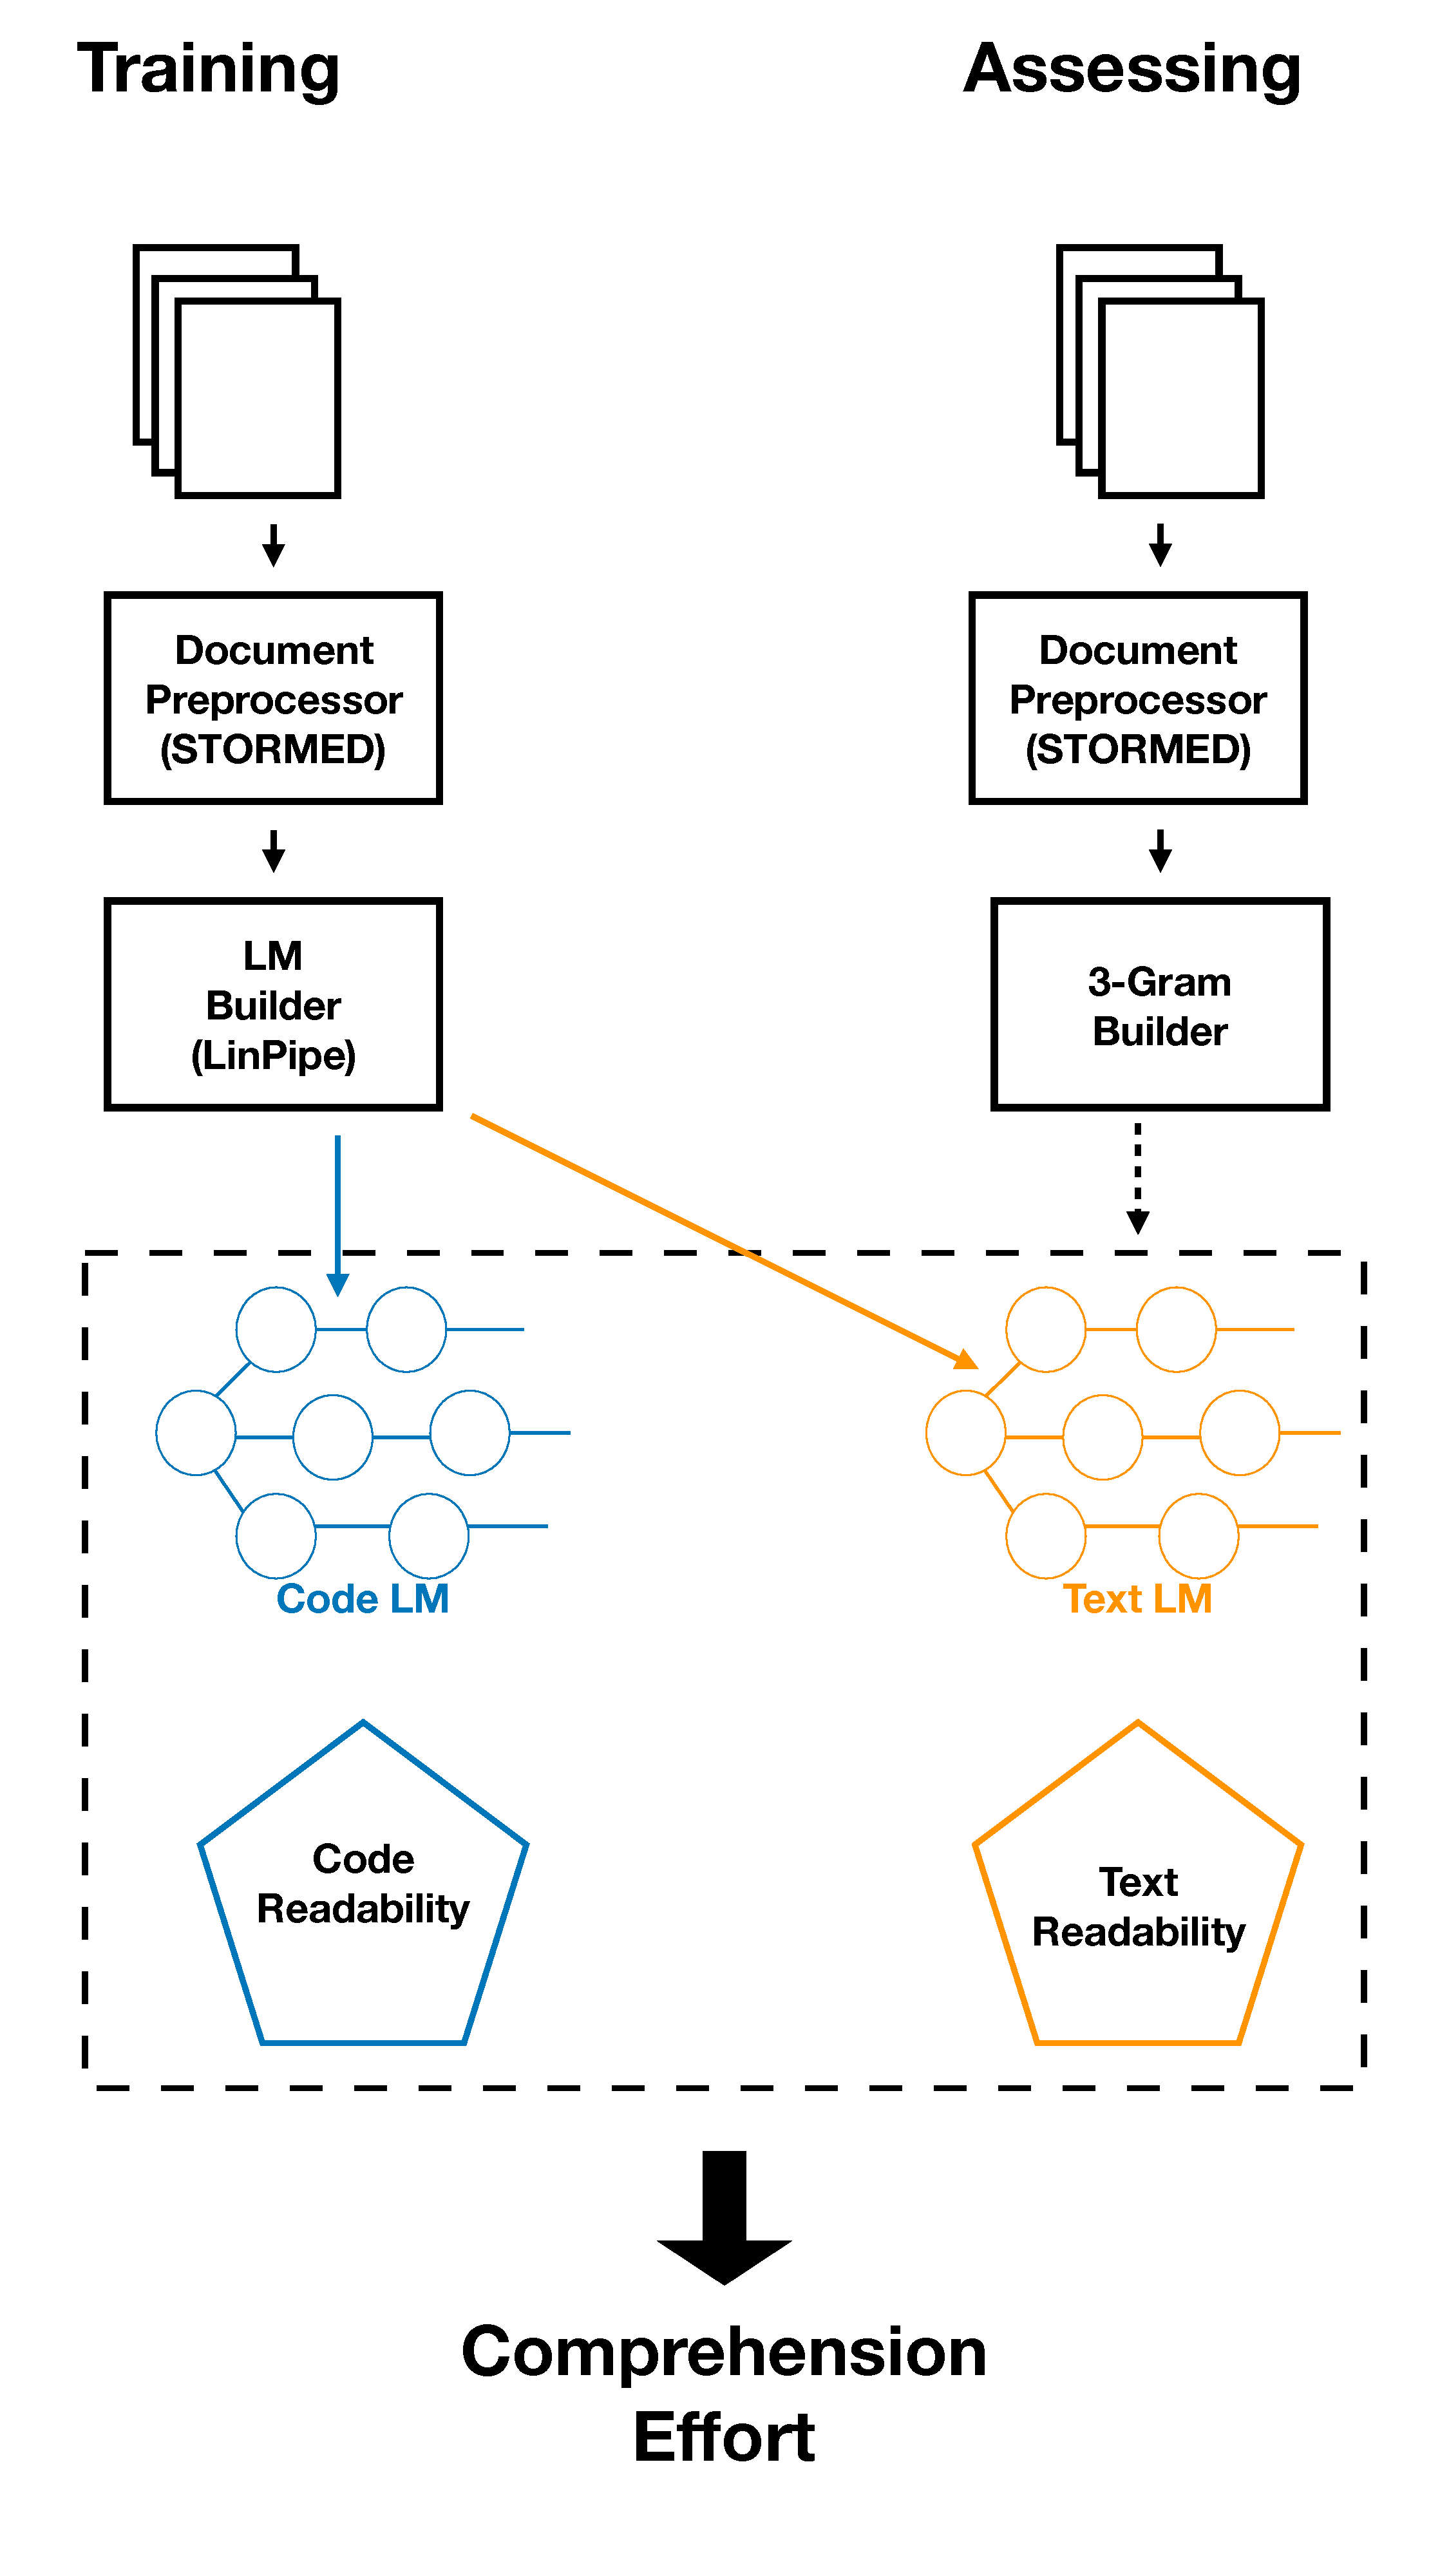
\includegraphics[width=6cm, height=10cm]{overview}
	\caption{Overall architecture of our approach}
	\label{overview}
	\end{figure}
	
	\section{Overview}

	Fig \ref{overview} shows the overall architecture of our approach. As we can see, there are two \emph{language models}, one for code and one for text (natural language), and the whole process is divided in two phases that work in parallel: 
	\begin{itemize}

		\item \textbf{Training phase}: In this phase we train the language models on a given set of documents, where each document is broken down in two segments: code and text. To extract code and natural language from a document, we use Stormed Island Parser\footnote{\url{https://stormed.inf.usi.ch}} \cite{Ponz2015a}. The \emph{code language model} will be trained with the code segment, and the \emph{text language model} will be trained with the text segment. These language models will give us the familiarity of a given document in the assessing phase.


		\item \textbf{Assessing phase}: In this phase we give each document a \emph{Comprehension Effort} score. As a first step we use Stormed \cite{Ponz2015a} to brake down each document in two segments: code and text, then we use the language models that we trained in the training phase to estimate the familiarity. In the same time we use Flesch$-$Kincaid\cite{Kincaid} to calculate the text readability, and RayKernel \cite{Buse:2010:LMC:1850489.1850615} to calculate the code readability. In the last step we combine the familiarity and the readability to get the comprehension effort.
	
	\end{itemize}

	In the next sections we explain the training and assessing phase, and we give more details about the component that are used in the whole process.

	\section{Training Phase}

	As we have mentioned before, in the training phase we use Stormed to distinguish between code and text, and we train two language models, one for text and one for code. We explain what Stormed is and how we use it, and then we explain what a language model is, and how we train it.

	\subsection{Stormed Island Parser}
	
	 Stormed is a dataset and parser for Stack Overflow that models the posts by building a heterogeneous abstract syntax tree (H-AST) for each discussion in the data dump \cite{Ponz2015a}.
	 \subsubsection{Stormed Parser}
	 Stormed can parse any given data in form of text. For example, given the following text : 
	 \begin{verbatim} With a sorted array, the condition data[c] >= 128  \end{verbatim} 
	 Stormed can identify  \emph{``With a sorted array, the condition''} as text, and \\``$data[c] >= 128$'' as code. 


	 Stormed gives us more detailed information about the code, that can be one of the following possible structured fragments:
	 \begin{itemize}
	 \item \textbf{JavaASTNode}: Java code including incomplete fragments.
	 \item \textbf{StackTracesASTNode}: Stack traces including incomplete stack trace lines.
	 \item \textbf{XMLASTNode}: XML/HTML documents, tags and elements.
	 \item \textbf{JSONASTNode}: JSON fragments.
	 \end{itemize}

	 \subsubsection{Stormed Dataset}

	  As shown in Fig \ref{stackOverflow} each Stack Overflow document is represented with HTML tag, Stormed extracts two types of information units:
	 	 \begin{itemize}
		\item \textbf{Natural Language Tagged Unit} is the textual part of a discussion. Text units are all fragments that are not tagged as <code> or <pre><code>.	
		\item \textbf{Code Tagged Unit} is the code part of a discussion. Structured Fragment Unit are every contents tagged as <code> or <pre><code>.
	 \end{itemize}


	\begin{figure}[htbp]
	 \centering
	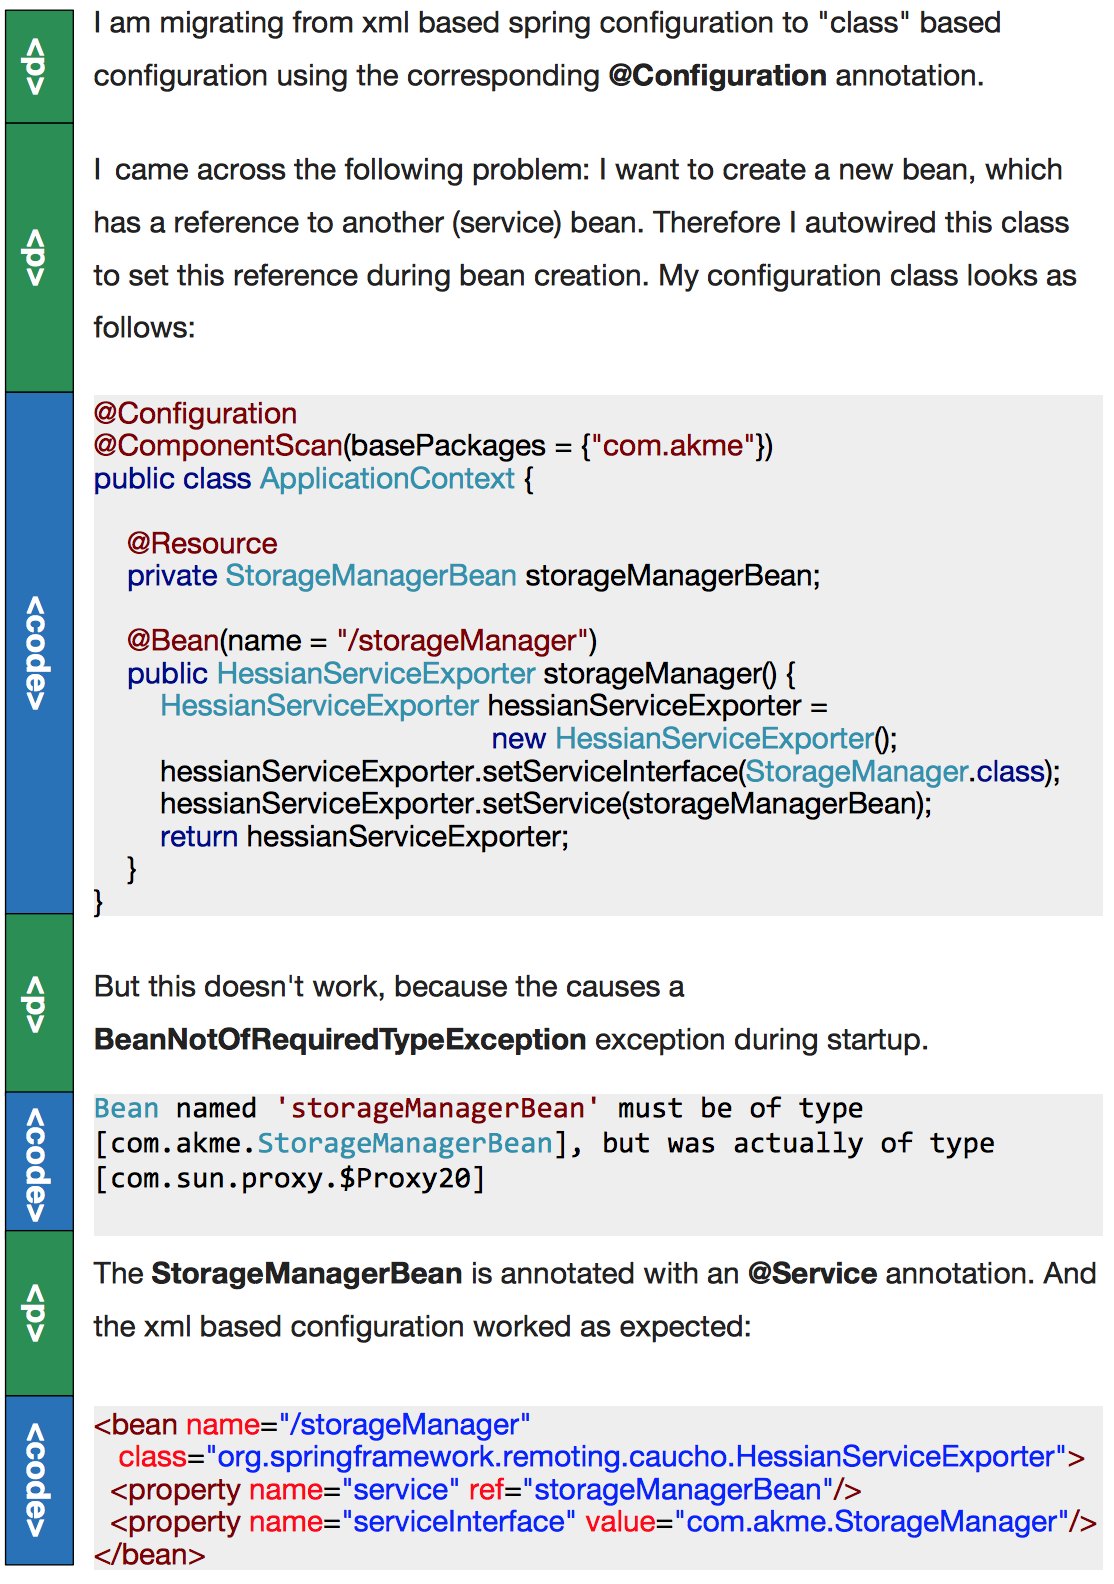
\includegraphics[width=6cm,height=8cm]{stackOverflow}
	\caption{Example of Stack Overflow question with HTML tagging}
	\label{stackOverflow}
	\end{figure}

	% \begin{figure}[htbp]
	% \centering
	% 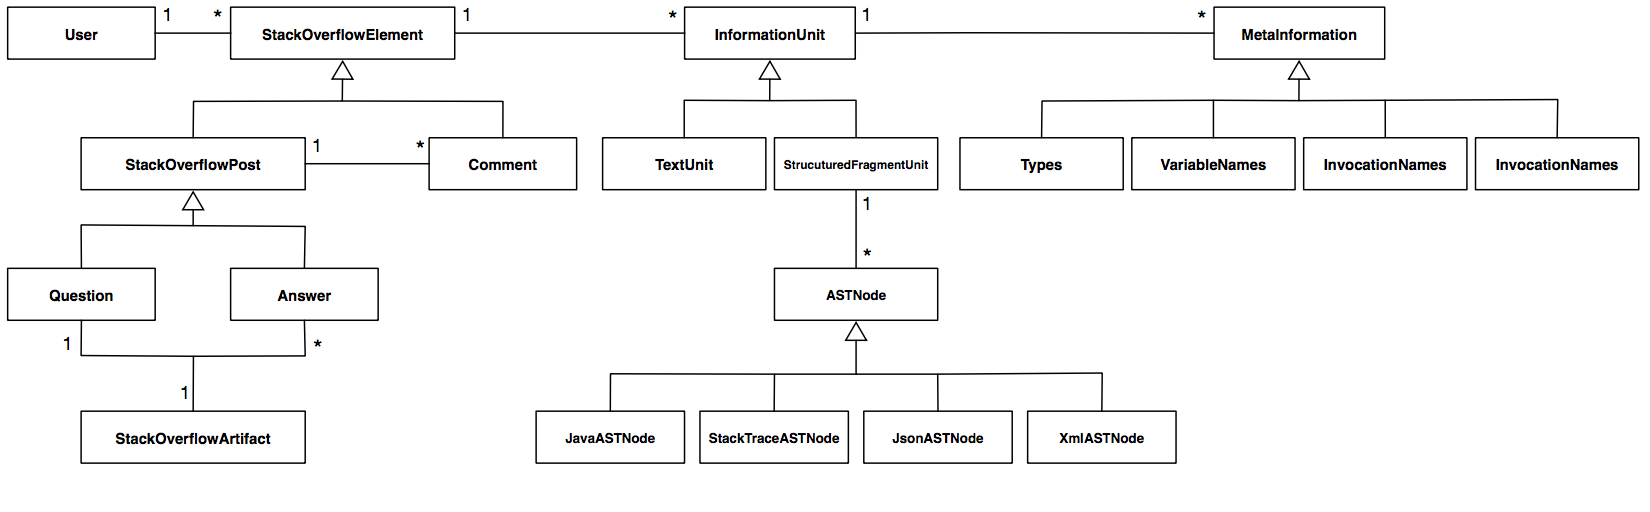
\includegraphics[width=\textwidth,height=5cm]{stormed}
	% \caption{Stormed Object Model of the dataset}
	% \label{stormed}
	% \end{figure}

	The extracted units are modeled as a H-AST, and added to the data set. The Stormed data contains a set of JSON files, one for each Stack Overflow discussion. The JSON files can be parsed to obtain objects corresponding to the H-AST. \\

	
	Stormed allows us to distinguish between the textual part (natural language), and the code part. Moreover, Stormed parses the code part and identifies the Java code even if the code is incomplete.

	\subsection{Language Model}

	A \textbf{Probabilistic Language Model (LM)} is a probability distribution over sequences of words. Given such a sequence of length m, it assigns a probability $P(w_{1},\ldots ,w_{m})$ to the whole sequence\footnote{\url{https://en.wikipedia.org/wiki/Language_model}}.\\
	The goal of the language model is to compute the probability of a sentence or sequence of words.
	\[P(W) = P(w_{1},w_2,w_3,w_4,w_5\dots w_n)\]
	A LM can also compute the probability of an upcoming word.
	\[P(w_5|w_1,w_2,w_3,w_4)\]
	A LM applies Markov Chain Assumption to compute $P(W)$
	\[P(w_1w_2\dots w_n) \approx \prod_{i} P(w_i|w_{i-k} \dots w_{i-1})\]
	Each component in the product is approximated
	\[P(w_i |w_1w_2\dots w_{i-1}) \approx P(w_i |w{i-k} \dots w_{i-1})\]
	\textbf{Bigram model} provides the conditional probability of a word given the previous word.
	\[P(w_i |w_1w_2 \dots w_{i-1})\approx P(w_i |w_{i-1})\]
	The bigram model can be extended to trigrams, 4-grams, 5-grams, \dots , n-grams.\\
	$P(w_i |w_{i-1}$ is the maximum likelihood estimation in a bigram where 
	\[P(w_{i}|w_{{i-1}})=\frac{count(w_{{i-1}},w_{i})} {count(w_{{i-1}})}\]
	\textbf{Example}\\
	Lets consider the following text:
	\begin{verbatim}
	Hi I am John
	Hi John I am David
	Hi I am looking for John
\end{verbatim}
	\[P(I|HI)\ = \frac{2}{3} = 0.67\]
	The probabilities of the sentence ``I like Italian food'' estimated by a bigram model is:
	\[P(like|I) \times P(Italian|like) \times P(food|Italian)= 0.00042\]
	To avoid underflow and to make multiplication faster, we use log space.
	\[log( p_1 \times p_2 \times p_3 \times p_4 ) = log (p_1) + log (p_2) + log (p_3) + log (p_4)\]



	\subsection{Training the Language Model}
	In our approach we use the 3-Gram model, we tried the 4-Gram and the 5-Gram but there was no significant difference. As we said before, we differentiate between natural language and code, therefore, we create a language model for each as we can see in Fig \ref{trainingLm}.\\

	\begin{figure}[H]
	\centering
	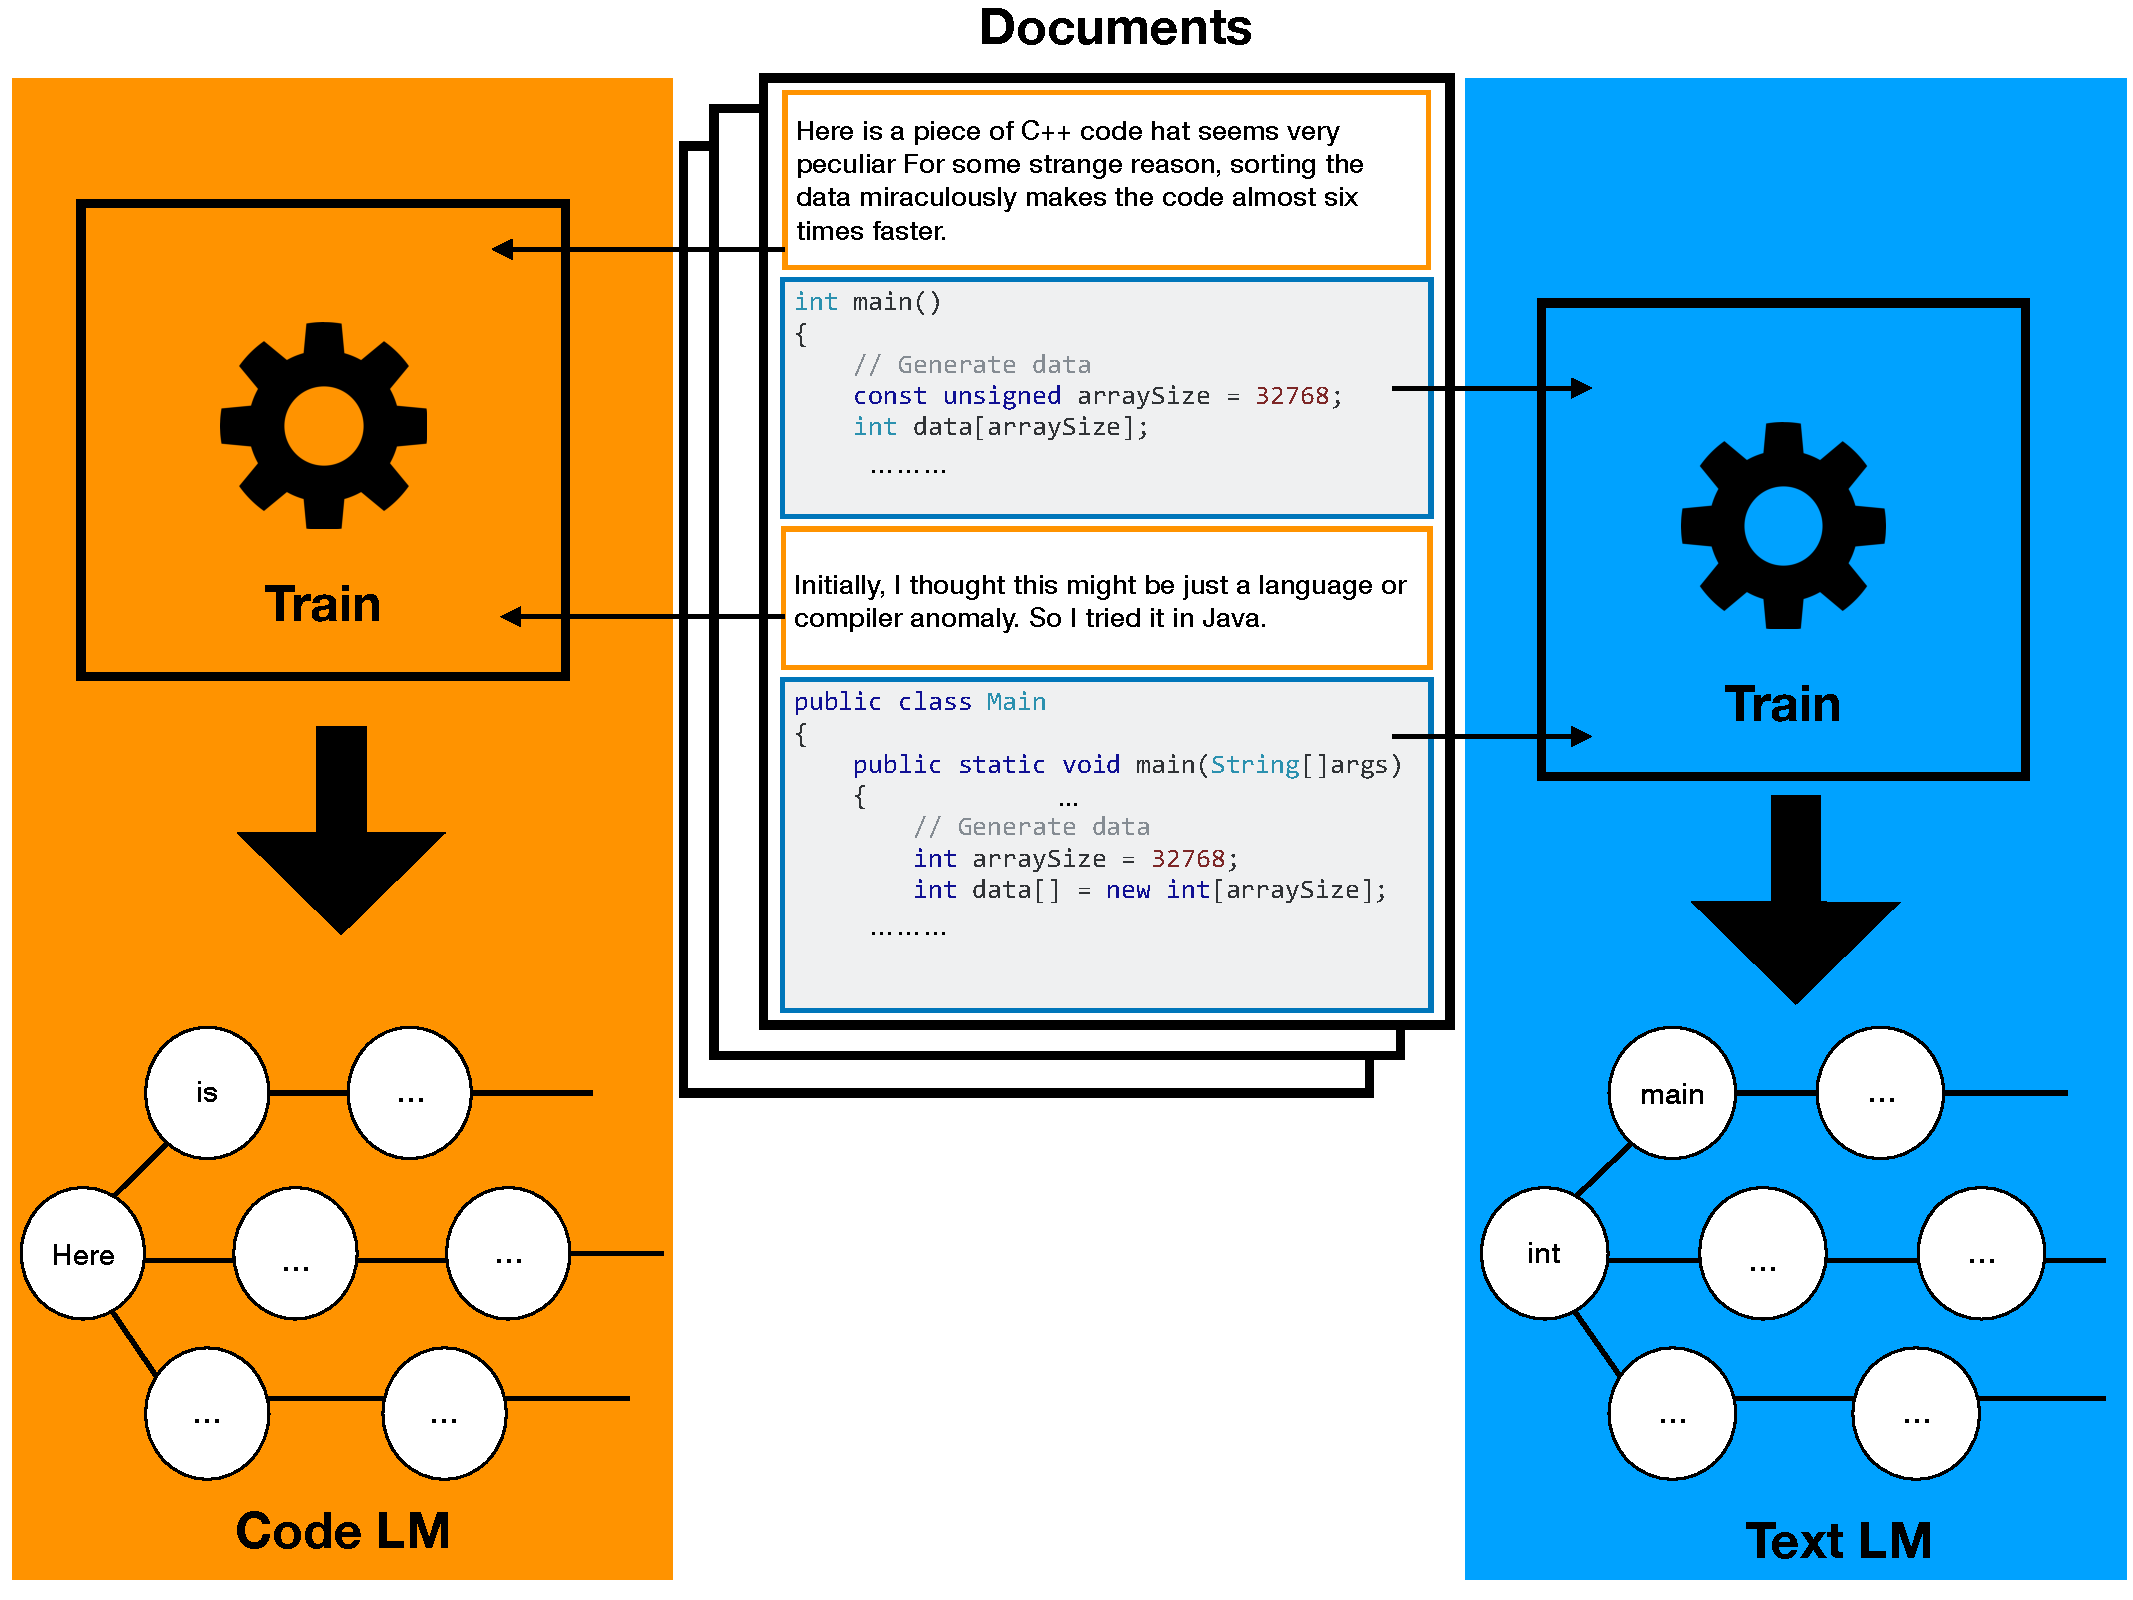
\includegraphics[width=\textwidth]{trainingLm}
	\caption{Training Language Model overview}
	\label{trainingLm}
	\end{figure}


	\begin{itemize}
		\item \textbf{Natural Language LM training}: Once we have identify the textual part of a document, we remove the stop words, since they are common words and they add noise to the LM, then we train the \emph{Natural Language LM} with the filtered text.
		\item \textbf{Code LM training}: For the code part we use a similar approach. We use ANTLR\footnote{\url{http://www.antlr.org}} parser to parse the code and to create tokens that we model as 3-Grams, and we pass them to the LM. But before training the LM on the code we remove all separators Fig \ref{FilterLM}.


		The reason why we decide to remove separator is because given a code with three nested loops:	

		\begin{lstlisting}
for(int a in list){
	for(int b in list){
		for(int c in list){
			System.out.println(a + b + c)
		}
	}
}

		\end{lstlisting}

		The code ends with three curly brackets $\textbf{\}\}\}}$ that form the most popular 3-Gram since it is frequent to have a sequence of brackets or parentheses in code. We had several situation where the most familiar 3-Gram was three brackets, for this reason we decide to remove this noise by filtering the separators.

	\end{itemize}
	

	\begin{figure}[htbp]
	\centering
	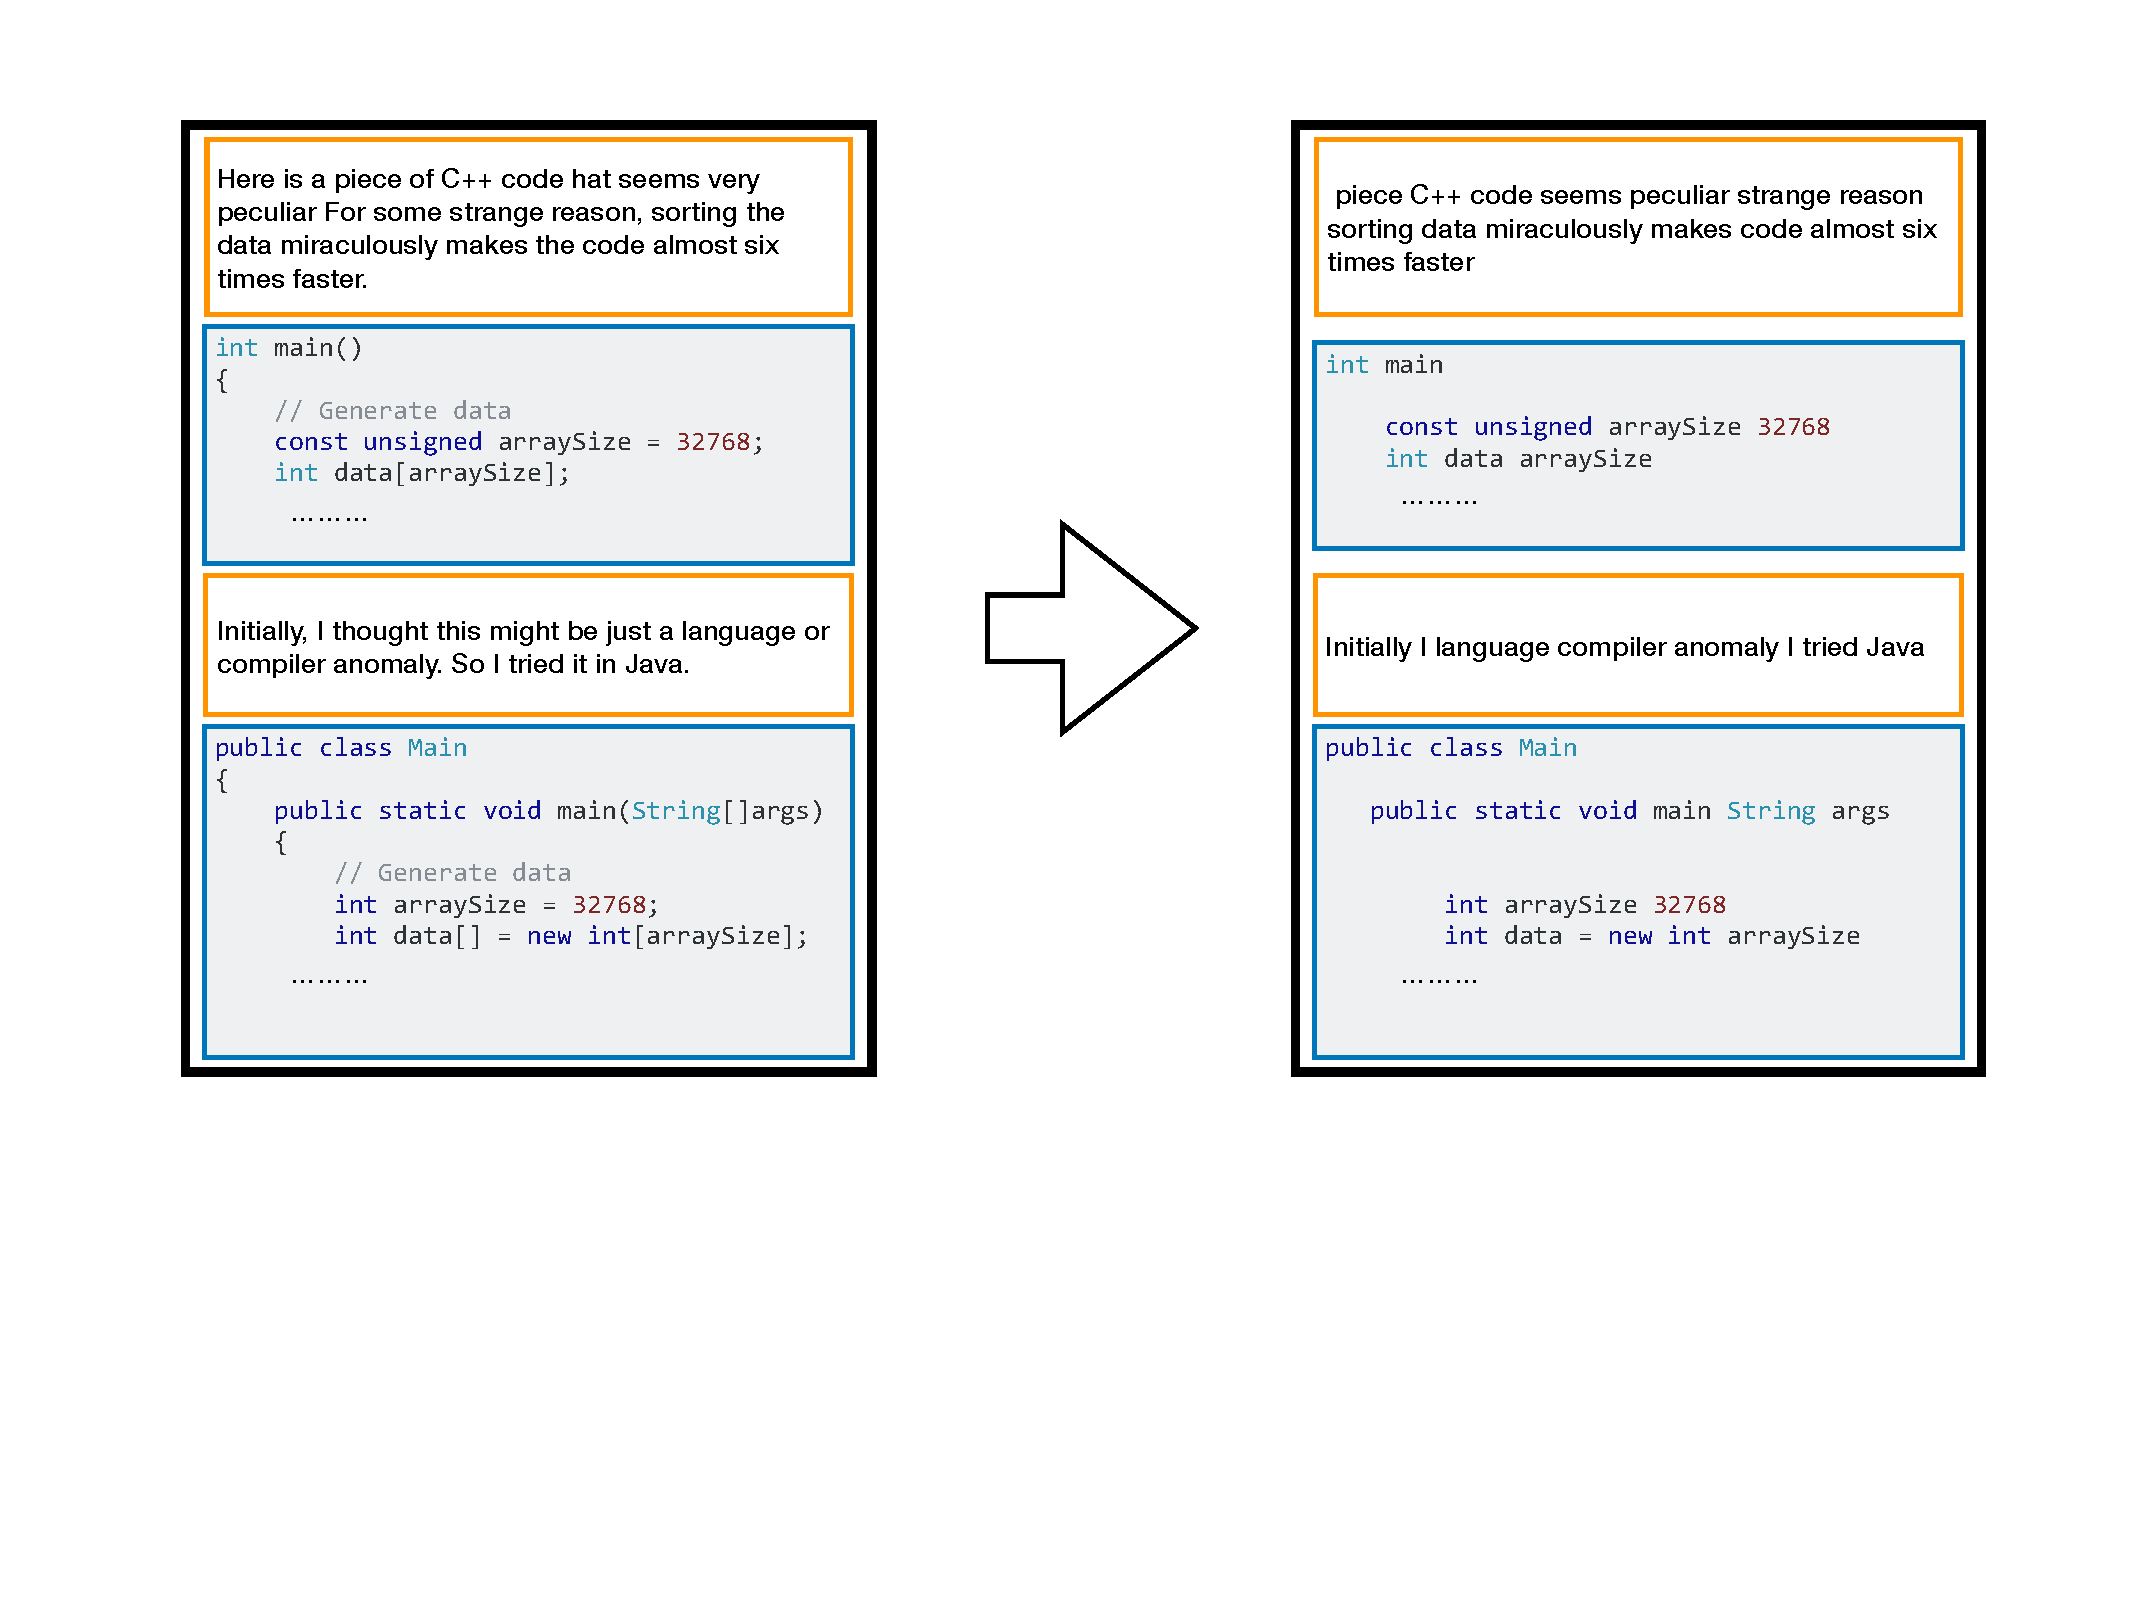
\includegraphics[width=\textwidth]{FilterLM}
	\caption{Filtering stop words and separators}
	\label{FilterLM}
	\end{figure}

	\newpage

	\section{Assessing Phase}

	In the assessing phase we estimate the familiarity of a given document, then we calculate the document readability and we combine them in a comprehension effort score.


	\subsection{Familiarity Estimation}
	We define the familiarity as the estimation of likelihood of a specified character sequence. But before estimating the familiarity, we need to do the following preprocessing steps:
	\begin{itemize}
		\item \textbf{Selecting \& Filtering}: As we did in the training phase, we use Stormed Island Parser\footnote{\url{https://stormed.inf.usi.ch}} \cite{Ponz2015a} to break down a document into text and code. We remove the stop words form the text, we parse the code\footnote{\url{http://www.antlr.org}} and we remove the separators, as shown in Fig \ref{FilterLM}
		\item \textbf{3-Grams generating }: In Fig \ref{3gram-evaluating} we can see that each chunk of code or text is transformed to a 3-Gram model, and then the language model evaluates the familiarity of each N-Gram.
			
			% \begin{figure}[htbp]
			% \centering
			% 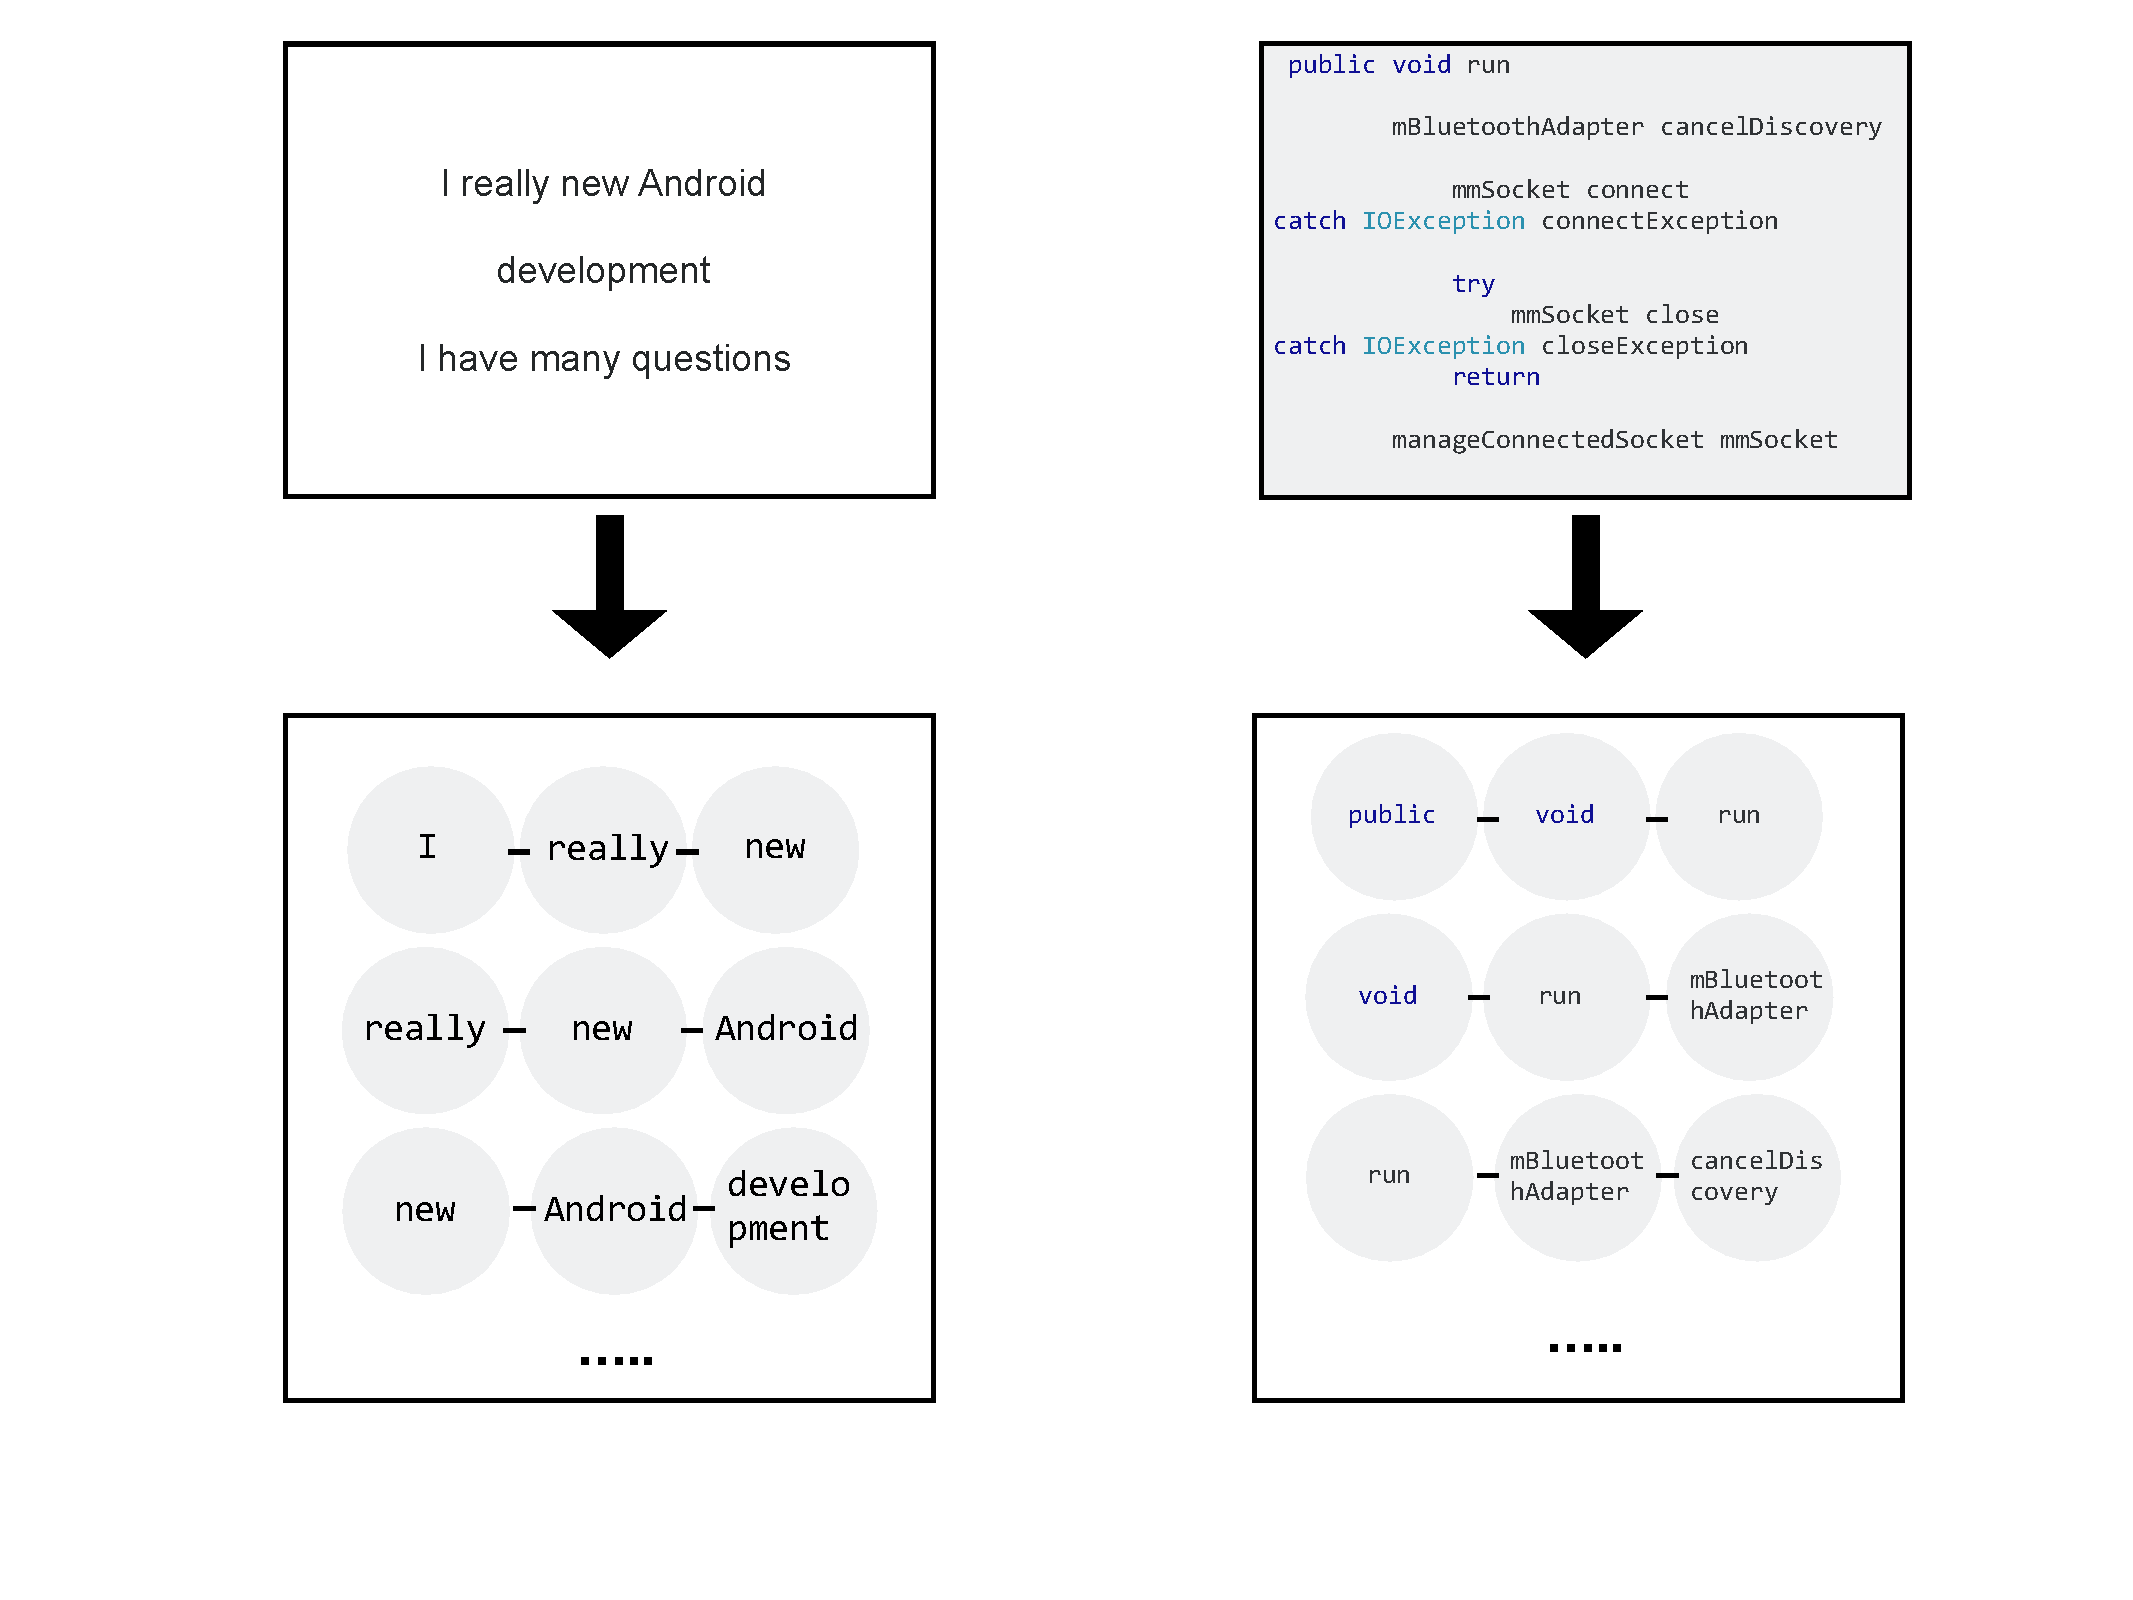
\includegraphics[width=\textwidth]{3gram-generating}
			% \caption{3-Gram generating process}
			% \label{3gram-generating}
			% \end{figure}

			\begin{figure}[htbp]
			\centering
			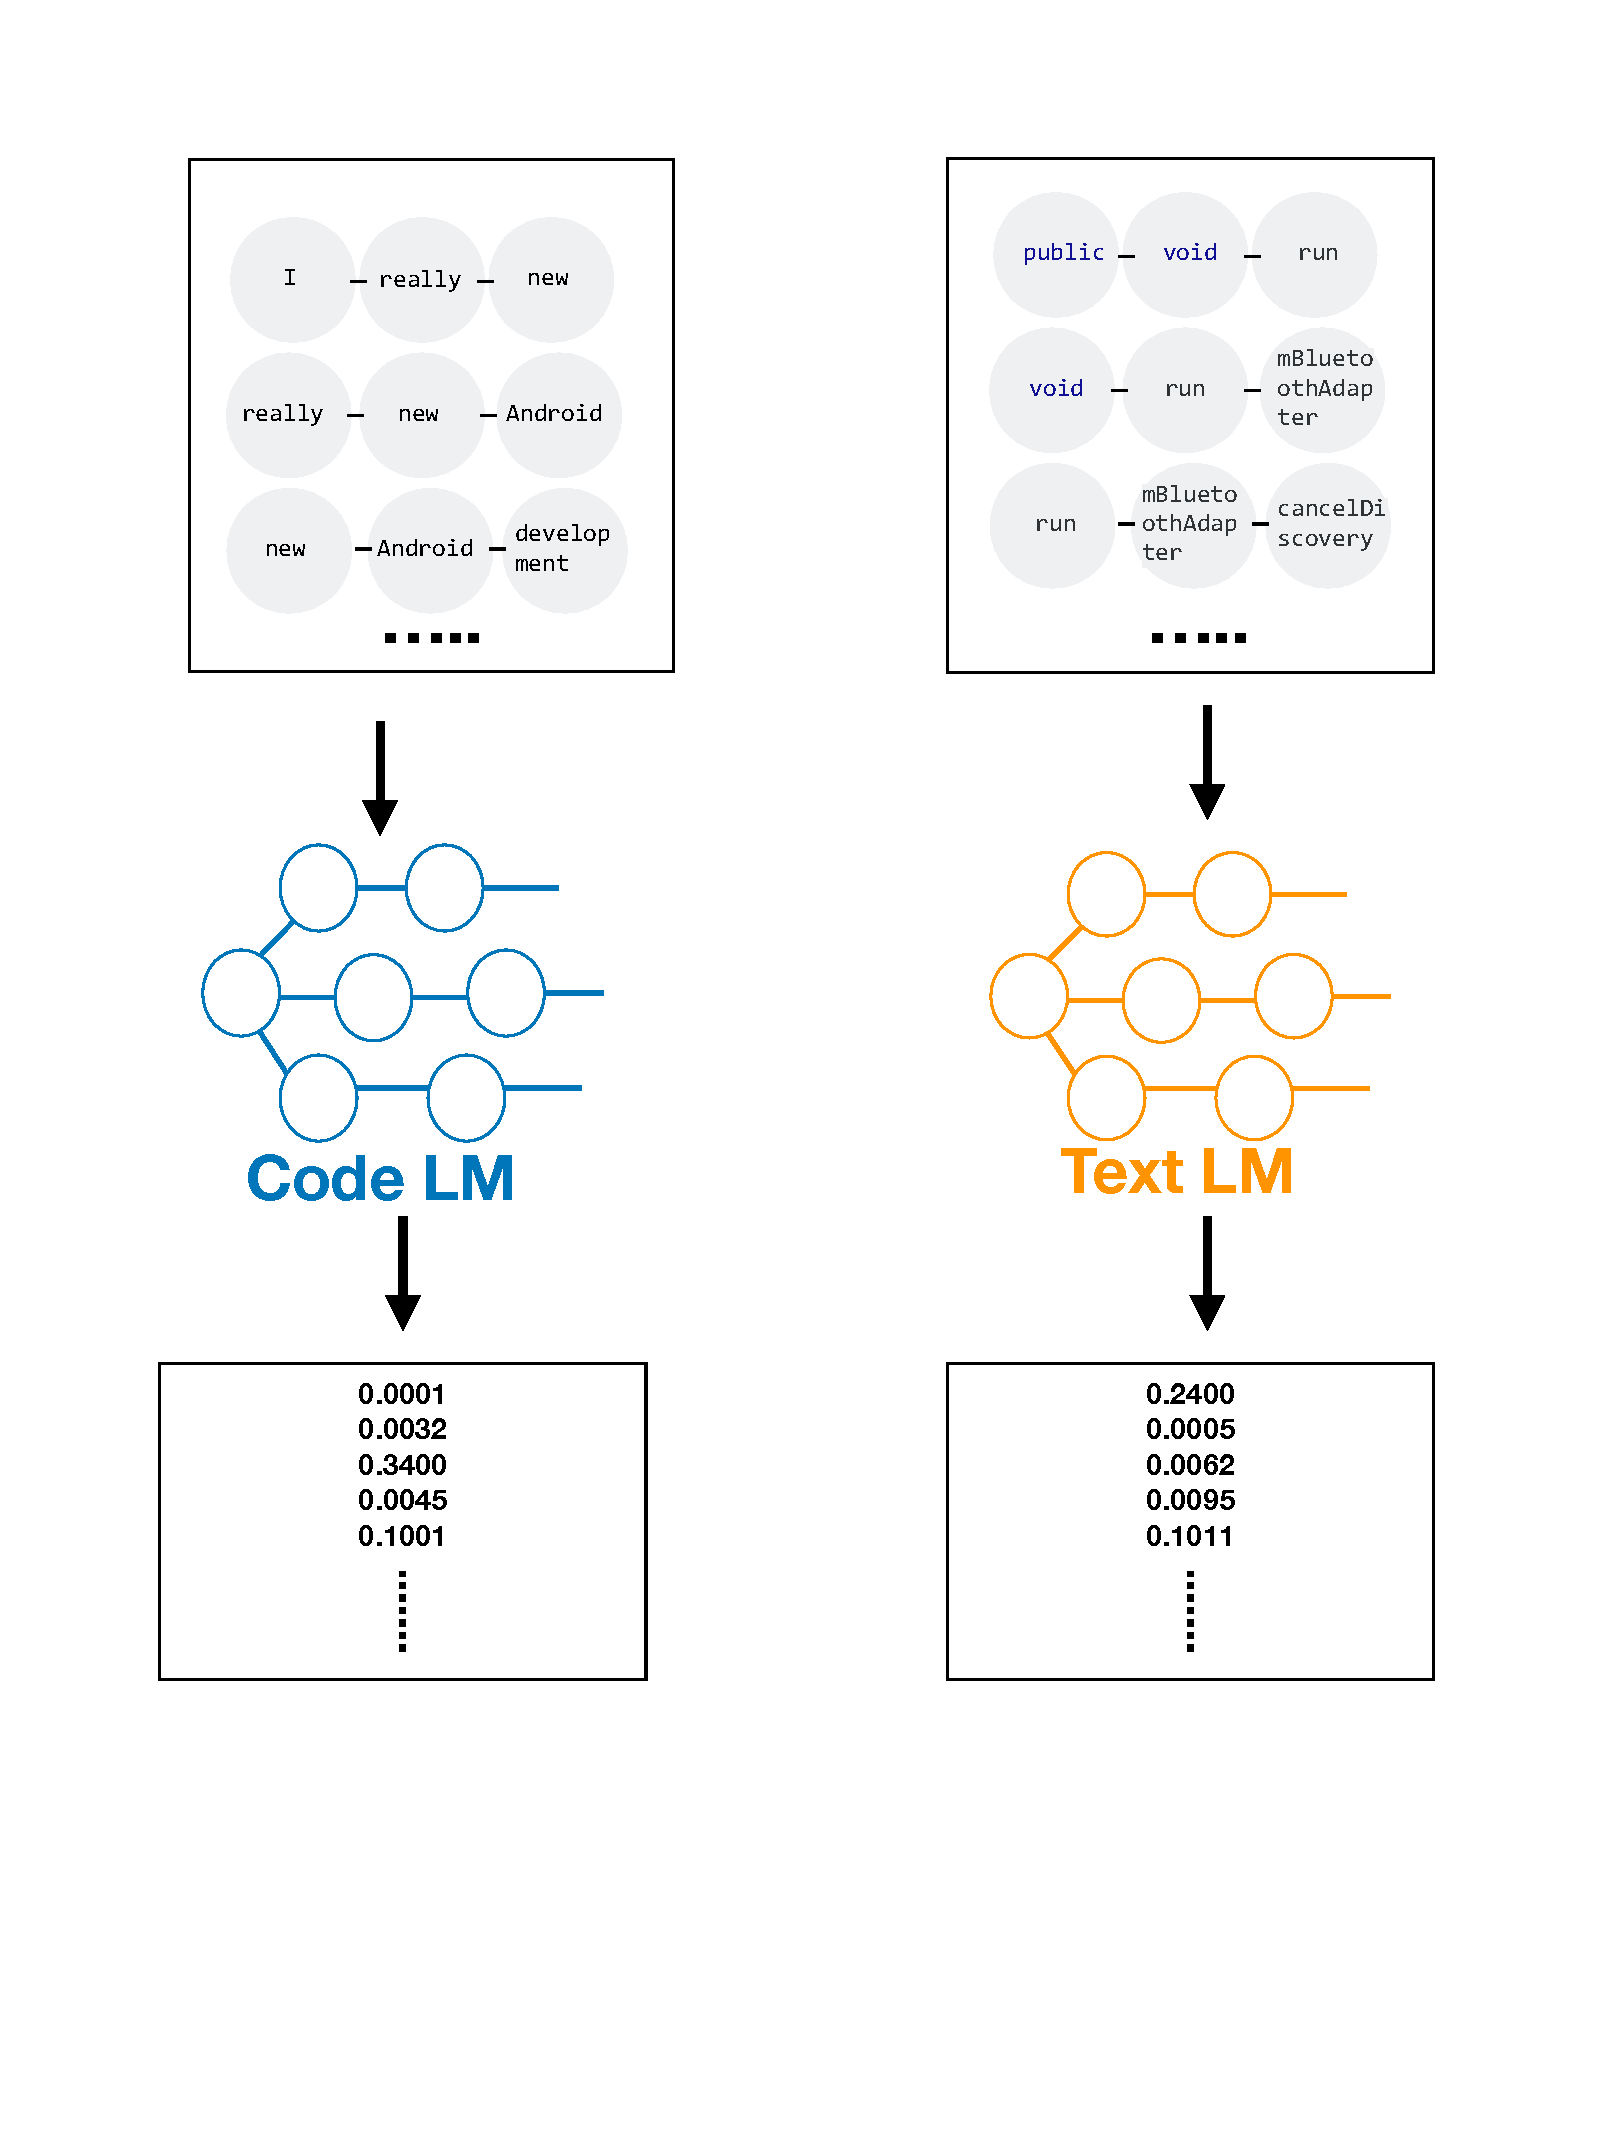
\includegraphics[width=\textwidth]{3gram-evaluating}
			\caption{3-Gram evaluating process}
			\label{3gram-evaluating}
			\end{figure}	
	
	
		\item \textbf{Familiarity aggregation}: Now that we have retrieved the familiarity of each 3-Gram of a given document, we need to aggregate them in one value. The trivial way is to multiply all the probabilities to get one value, but this approach is biased by the document length.\\
		As we can see in Fig \ref{aggregation-by-multiplication} we have 2 documents, a and b, where \emph{document b} contains twice the content of \emph{document a}. We expect that the familiarity in both documents must be the same since they have the same text, even though in \emph{document b} the text is duplicated.\\ 
			\end{itemize}
		\begin{figure}[H]
			\centering
			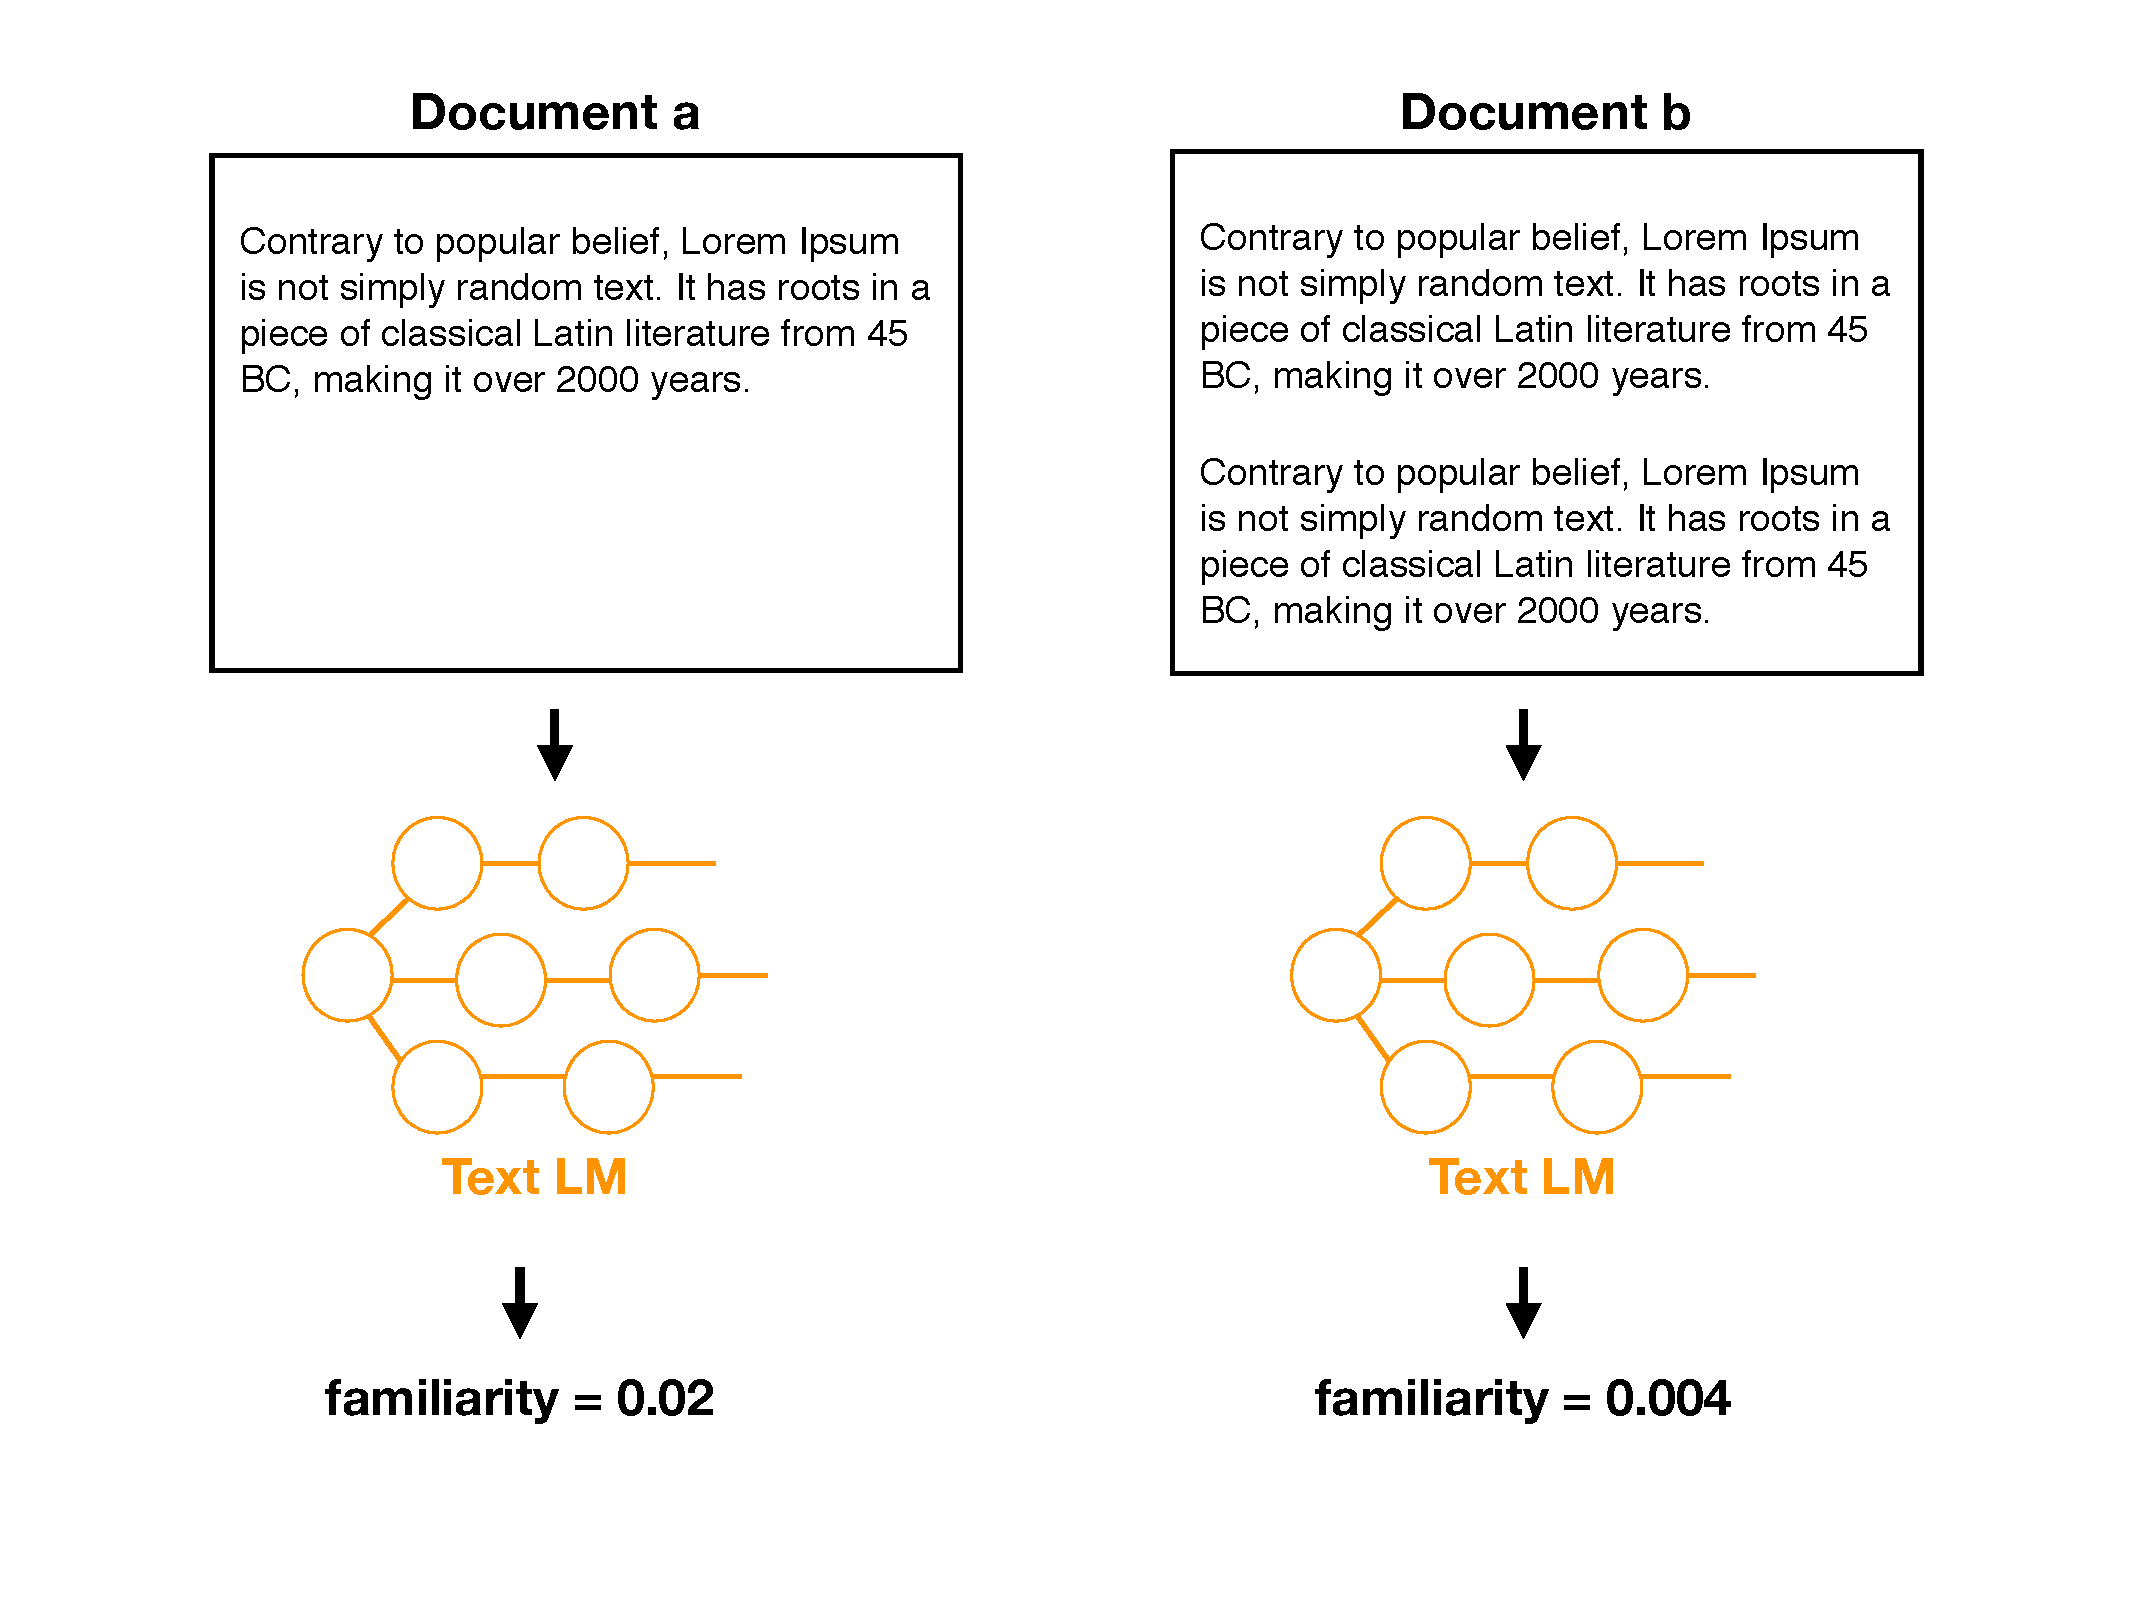
\includegraphics[width=\textwidth]{aggregation-by-multiplication}
			\caption{Aggregating probabilities by multiplication}
			\label{aggregation-by-multiplication}
			\end{figure}


			\begin{figure}[htbp]
			\centering
			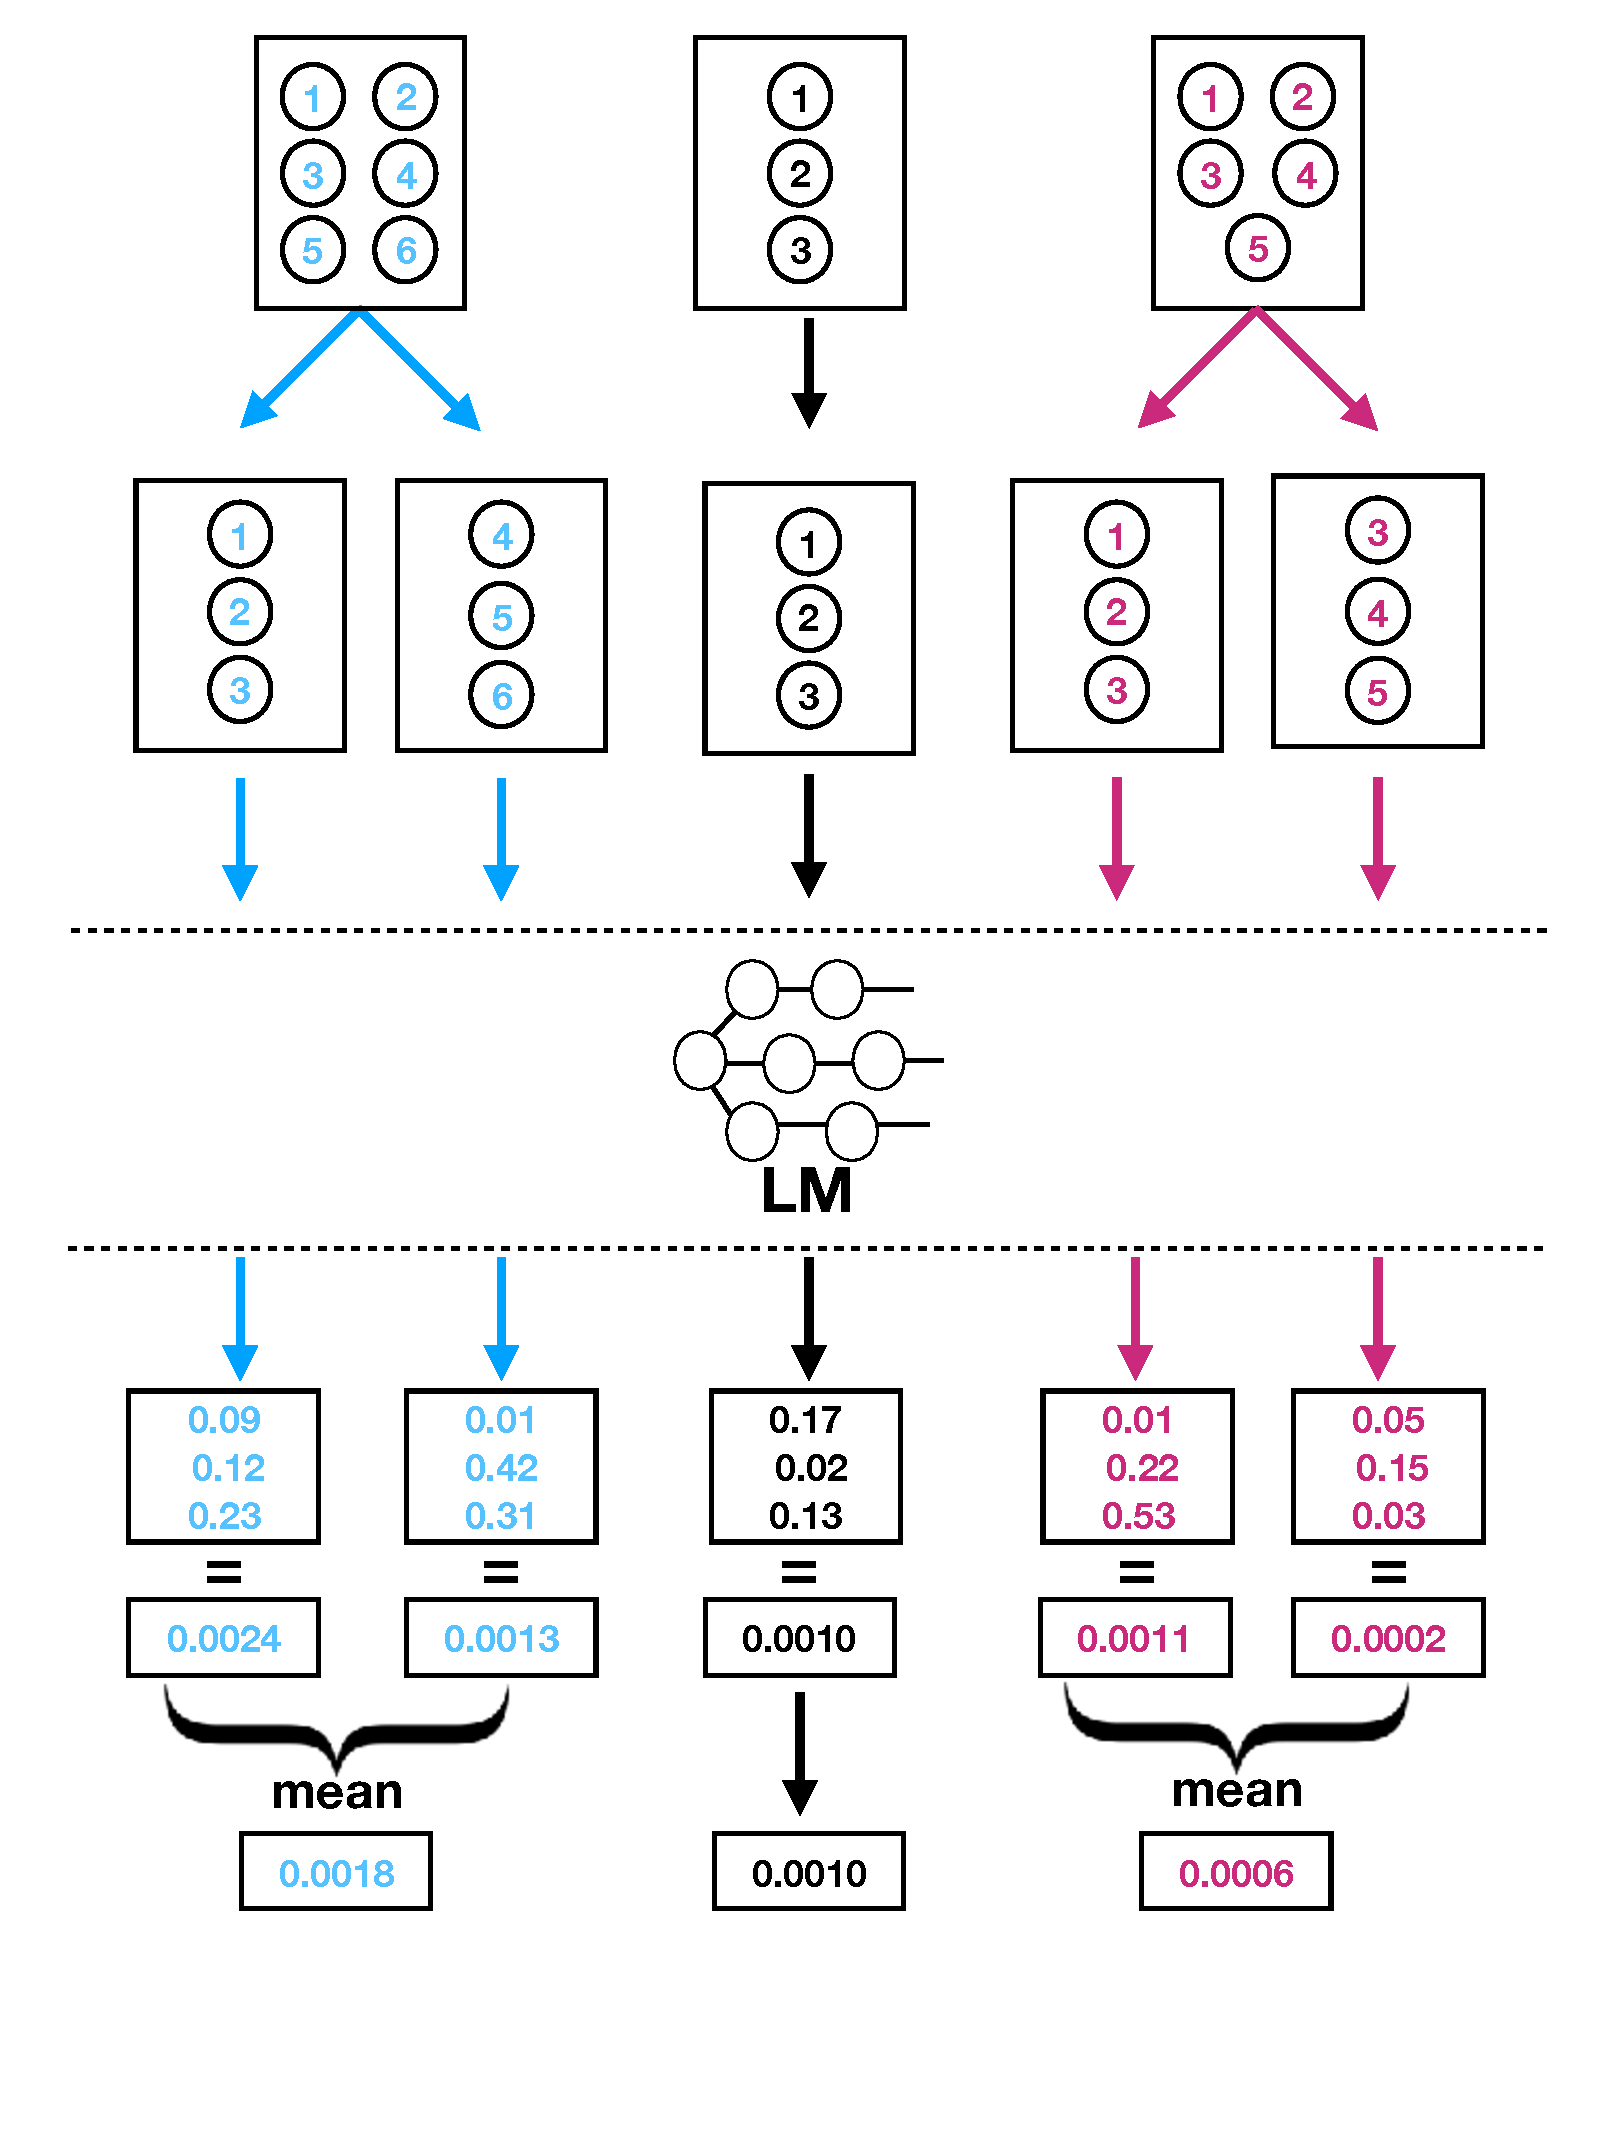
\includegraphics[width=\textwidth]{aggregation-by-mean}
			\caption{Aggregating probabilities by mean}
			\label{aggregation-by-mean}
			\end{figure}
		
		Given a set of documents with different length, the shortest documents turns out to be the most familiar. This approach is valid if all documents have the same length, which is not the case with the documents that we are dealing with, since they have heterogeneous length. 


		We tackle this problem by introducing a new approach to aggregate the probabilities as shown in Fig \ref{aggregation-by-mean}.
		The approach consists in 5 steps: 
		\begin{itemize}
			\item \textbf{step 1}: We select from the set the document with the smallest number of 3-Gram, say of length m.
			\item \textbf{step 2}: We split each document into chunks of length m.
			\item \textbf{step 3}: For each chunk we calculate the familiarity of its 3-Grams
			\item \textbf{step 4}: Now that all chunks have the same size, we calculate the familiarity of a chunk by multiplying the probability of all its 3-Grams
			\item \textbf{step 5}: Is the last step, we calculate the familiarity mean of each document chunks.
		\end{itemize}

	\subsection{Readability} 
		The document readability has a big impact on the comprehension effort. Two text documents can contain approximately the same information, but one text can be easy to read and the other one can be difficult to read, and it is the same for code. The following peace of code can be written in one line :

		\lstset{language=algebra,linewidth=0.95\linewidth,breaklines=true,
		basicstyle=\ttfamily,numberstyle=\tiny,escapeinside={//*}{\^^M},
		mathescape=true}
		\begin{lstlisting}
	{"name":"mkyong.com","messages":["msg 1","msg 2"],"age":100}

		\end{lstlisting}	
	But most likely developers will find it easier to read the indented code:\\

	 	\begin{lstlisting}
{
	"name":"mkyong.com",
	"messages":["msg 1","msg 2"],
	"age":100
}
	\end{lstlisting}
 
	As mentioned so far we distinguish between \emph{code readability} and \emph{text readability}. Therefore, we use different tools to calculate the readability of each. 

\subsection{Accounting for Text Readability}
	The text readability score is calculated by the \textbf{Flesch-Kincaid} \footnote{\url{https://en.wikipedia.org/wiki/Flesch–Kincaid_readability_tests}} formula:
	

	\[0.39\left({\frac  {{\mbox{total words}}}{{\mbox{total sentences}}}}\right)+11.8\left({\frac  {{\mbox{total syllables}}}{{\mbox{total words}}}}\right)-15.59\]
	A higher scores indicate that the document is easier to read, and a lower number indicates that the document is more difficult to read.\\ 
	Flesch-Kincaid score is scaled in 0-100 rage, but for convenience we normalize it to 0-1 range. The score can be interpreted as shown in the table below, Table \ref{tab:Flesch-Kincaid}.
	
	\begin {table}[H]
	\begin{center}
    \begin{tabular}{| l | l | p{7cm} | }
    \hline
    \textbf{Score} & \textbf{School Level} & \textbf{Notes} \\ \hline
    $100.0-90.0$ & 5th grade & Very easy to read. Easily understood by an average 11-year-old student.\\ \hline
    $90.0-80.0$ & 6th grade & Easy to read. Conversational English for consumers.\\ \hline
 	$80.0-70.0$ & 7th grade & Fairly easy to read. \\ \hline
	$70.0-60.0$ & 8th \& 9th grade & Plain English. Easily understood by 13- to 15-year-old students.\\ \hline
	$60.0-50.0$ & 10th to 12th grade &  Fairly difficult to read.\\ \hline
	$50.0-30.0$ & College & Difficult to read.\\ \hline
	$30.0-0.0$ & College Graduate & Very difficult to read. Best understood by university graduates\\\hline

    \end{tabular}
	\end{center}
	\caption{Flesch-Kincaid score grade} \label{tab:Flesch-Kincaid} 
	\end{table}

\subsection{Accounting for Code Readability}
	To calculate the code readability we use \citet{Buse:2010:LMC:1850489.1850615} code readability metric, and tool\footnote{\url{http://www.arrestedcomputing.com/readability}}.
	 Buse and Weimer determined a set of code features that are predictive of readability. The features are listed in the Table \ref{tab:Buse and Weimer}.

	\begin {table}[H]
	\begin{center}
    \begin{tabular}{ | l | }
    \hline
    \textbf{Feature Name}\\ \hline
	line length (\# characters)\\ \hline
 	\# identifiers\\ \hline
 	identifier length\\ \hline
	indentation (preceding whitespace)\\ \hline
	\#keywords\\ \hline
	 \#numbers\\ \hline
	\#comments\\ \hline
	\#periods\\ \hline
	\#commas\\ \hline
	\#spaces\\ \hline
	\#parenthesis\\ \hline
	 \#arithmetic operators\\ \hline
	 \#comparison operators\\ \hline
	 \#assignments (=)\\ \hline
	 \#branches (if)\\ \hline
	 \#loops (for, while)\\ \hline
	 \#blank lines\\ \hline
	 \#occurrences of any single character\\ \hline
	 \#occurrences of any single identifier\\ \hline
    \end{tabular}
	\end{center}
		\caption{Buse and Weimer code features} \label{tab:Buse and Weimer} 
	\end{table}

	Buse and Weimer's readability score is scaled in 0-1 range, where a higher scores indicate that the code is easier to read and a lower number indicates that the code is more difficult to read.


\section{Accounting Comprehension Effort }

To calculate the \emph{Comprehension Effort} of a given document we calculate:
\begin{itemize}
\item The familiarity of the textual parts $f_{t}$ 
\item The familiarity of the code parts $f_{c}$
\item The readability of the textual parts $r_{t}$
\item The readability of the code parts $r_{c}$ 
\end{itemize}
 
 The $r_{t}$  and $r_{c}$ are on a scale of 0 to 1,  the $f_{t}$  and $f_{c}$ are unbounded $log_{2}$ probabilities.\\
 We propose two formulas to calculate the \emph{Comprehension Effort}:

 \[\text{Comprehension Effort = }\frac{(r_{c}\times f_{c}) + (r_{t} \times f_{t})}{2} \]
 In this formula the \emph{readability} and the \emph{familiarity} have the same weight in calculating the \emph{comprehension effort}
 \[\text{Comprehension Effort = }\frac{(r_{c}\times f_{c}) + (r_{t} \times f_{t})}{r_c+r_t} \]
 In this formula the \emph{familiarity} has a higher weight, but we decided to explore the first formula in this thesis and the second one in future research.
	
\chapter{Study Design}

	In this chapter we present two studies aimed of assessing the LM capability to evaluate the familiarity of a given document, and to evaluate the effectiveness of our approach in assessing documents by the comprehension effort. Towards this goal, we run two tailored studies:
	

	The first study evaluates the familiarity approach. In this study (Experiment-1) we select a set of Android documents representing the developer knowledge context, and we train the LMs with these documents (Chapter 3.2). Once we trained the language model, we evaluate the familiarity of a given set of documents about Android and other documents that are not related to Android (Chapter 3.3.1). 
		

	 The second study evaluates our approach in assessing documents by comprehension effort. In this study (Experiment-2) we ask developers to read a set of tutorials, and then we give them a set of documents, where some documents are related to the tutorials and some are not, and we ask them to score the documents comprehension effort on a scale from 1 to 5. Then we compare their score with our precomputed comprehension effort score (Chapter 3.4).


	\section{Research Questions}
	To evaluate the effectiveness of our approach we have formulated the following research questions:
	\newpage

	 \textbf{RQ1}: \emph{Can a language model correctly evaluate the familiarity of a given document?}


		We have answered this research question by downloading 200,000 Stack Overflow questions tagged as Android. From these 200,000 documents we select 5 training sets with different size (10, 100, 1000, 10000, 100000), and we select 1000 documents for testing.


		We extend the testing set by downloading: 
		\begin{itemize}
			\item 1000 Stack OVerflow questions tagged as JavaScript.
			\item 1000 Stack OVerflow questions tagged as Swift.
			\item 1000 Stack OVerflow questions tagged as Java.
		\end{itemize}

		We create a code LM and a text LM, and we train them with the Android 10 documents training set, then we calculate the familiarity of the testing sets
		(Android, JavaScript, Swift, Java). We repeat this experiment with 100, 1000, 10000, 100000 android training sets to understand how the training set size can influence the performance. Then we plot the familiarity results to check if the LMs classify Android documents as the most familiar.\\


		{\textbf{RQ2}: \emph{What is the accuracy of our technique in assessing documents by the comprehension effort?}


		To answer this research question we asked two developers who has no experience with Android to read a set of introduction tutorials to Android, then we asked them to read two Android tutorials, the first one explains how to use the \emph{Android-Bluetooth} API and the second one explains how to use the \emph{Android-Camera} API. Once they have finished reading the tutorials we asked them to score the comprehension effort of 6 documents from Stack Overflow. The comprehension effort scores are on a scale from 0 to 5, where a higher score indicates a higher effort in comprehending the documents. The developers scored the following 6 documents:

		\begin{itemize}
			\item   Android-Bluetooth discussion\footnote{\url{https://stackoverflow.com/questions/9693755}}.
			\item   Android-Camera discussion.\footnote{\url{https://stackoverflow.com/questions/5991319}}
			\item   Android-AsyncTask discussions (not related to \emph{Bluetooth} or \emph{Camera}) \footnote{\url{https://stackoverflow.com/questions/31874990}}.
			\item   Android-Database discussions (not related to \emph{Bluetooth} or \emph{Camera})\footnote{\url{https://stackoverflow.com/questions/17451931}}.
			\item   2 Cordova discussions. (Cordova also known as PhoneGap is a mobile application development framework that enables software developers to build applications for mobile devices using CSS3, HTML5, and JavaScript)\footnote{\url{https://stackoverflow.com/questions/20835768}} \footnote{\url{https://stackoverflow.com/questions/10023328}}.
		\end{itemize}

		We train the LMs with the tutorials that we gave to the developers. Since the tutorials are not enough to train a LM, we augment the set by adding several tutorials that have the same subject as the one that we gave to the developers. We also train the code LM with as set of \emph{Android-Bluetooth} and \emph{Android-Camera} code snippets from \emph{Gist}\footnote{\url{https://gist.github.com/}}.


		 After the training phase we calculate the comprehension effort of the 6 Stack Overflow documents and we compare our results with the developers scores.



	\section{Data Collection}	

	To run the two experiments we collect and extract data from different sources. In the next sections we explain how we collect data for each experiment.

	\subsection{Experiment-1}

	Stormed dataset provides us with a set of JSON files, one for each discussion. We use Stormed development kit to parse the JSON files and obtain objects corresponding to the H-AST.
	As we mentioned in the previous section, in Experiment-1 for the training set we select a set of 100,000 Android discussions, and for the testing set we select a set of 1000 Android discussions. These sets are retrieved from the Stormed dataset, where we select discussions that are tagged only as Android, and the training and testing sets are disjoint.

	We also use Stack Overflow dump\footnote{\url{https://archive.org/details/stackexchange}} to select the JavaScript, Swift and Java discussions that we add to the testing set. We selected Java discussions that are not also tagged as Android to avoid having Android discussions in the Java set, since Android is implemented in Java.

	\subsection{Experiment-2}
	
	In Experiment-2 we have a set of 4 tutorials that introduce Android to developers, and give them an overview of how Android works. These tutorials are  selected from the \emph{tutorialspoint} website\footnote{\url{https://www.tutorialspoint.com/android/}}. 

	To augment the training set we select 4 Android introduction tutorials, 7 \emph{Android-Bluetooth}, 6 \emph{Android-Camera} tutorials from several websites. The tutorials are parsed by Stormed and passed to the LMs.  

	Besides the Android tutorials, we augment the training set by selecting from Gist 525 \emph{Android-Bluetooth}, 2666 \emph{Android-Camera} code snippets.

 	\section{Replication Package}

 	The Stormed data set that contains the Stack Overflow dump is available on Stormed website : \url{https://stormed.inf.usi.ch}.\\


 	The Thesis work is publicly accessible on this link : \url{https://github.com/talalelafchal/familiarity/tree/Aggregation}. The repository contains:
 	\begin{itemize}
 	\item Testing and training sets used in Experiment-1
 	\item Tutorials, Stack Overflow discussions and Gist files used in Experiment-2
 	\item Experiment-1 results in \emph{.csv} files with the R script to plot the results.
 	\item Experiment-2 results.
 	\item The source code.
 	\end{itemize} 


\chapter{Results}
	In this Chapter we present and discuss the evaluation results of our familiarity and comprehension effort estimating approach.

\section{Familiarity Estimation Results}

To evaluate our approach in estimating familiarity, we train two LMs (one for code and one for text) on a set of Android discussions from Stack Overflows' dump (training set). Then we evaluate the familiarity of 1000 Stack Overflow discussions on each of the following subjects: Android, Java, Swing and JavaScript.

We select 5 training sets with different size (10, 1000, 1000, 10000, 100000) to understand how the training set size can influence the performance. In the following sections we discuss the code LM results and the text LM results.

\subsection{Code LM Results}
  As a first step in the experiment, we train the code LM with 10 Android documents and we evaluate the code familiarity of the testing set. In Fig \ref{code10}, we show the box plot result. The $y$ axis represents the \emph{Log} estimated familiarity, where a higher box position indicates a lower familiarity. In this plot we can see that JavaScript and Swing documents are estimated as more familiar than Android documents. The reason why Android is not estimated as the most familiar is because 10 documents are too few to train a LM. 



\begin{figure}[H]
			\centering
			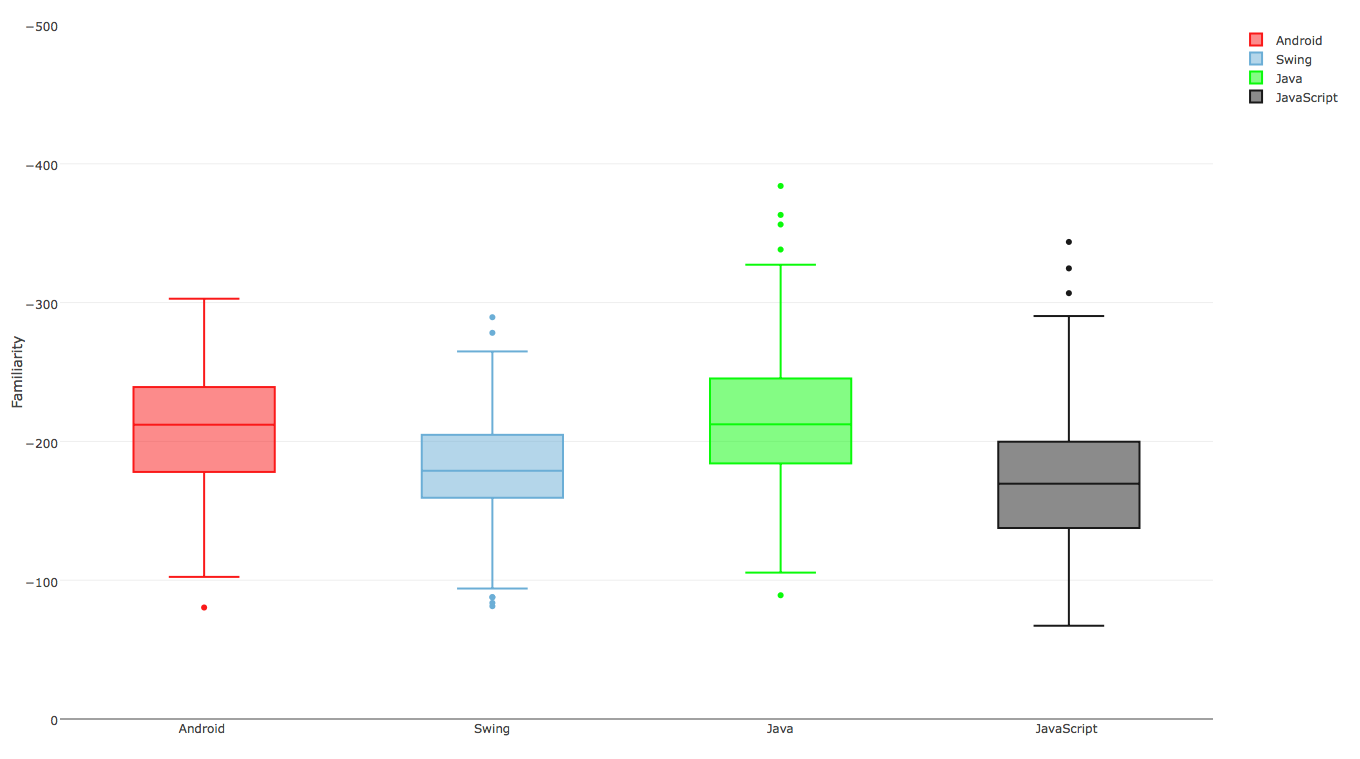
\includegraphics[width=\textwidth]{code10}
			\caption{Code LM trained with 10 documents}
			\label{code10}
			\end{figure}

Then we train the code LM with 100 Android documents, and as we can see in Fig \ref{code100}, the Android testing documents are not estimated as the most familiar, since 100 documents are still not enough.

\begin{figure}[H]
			\centering
			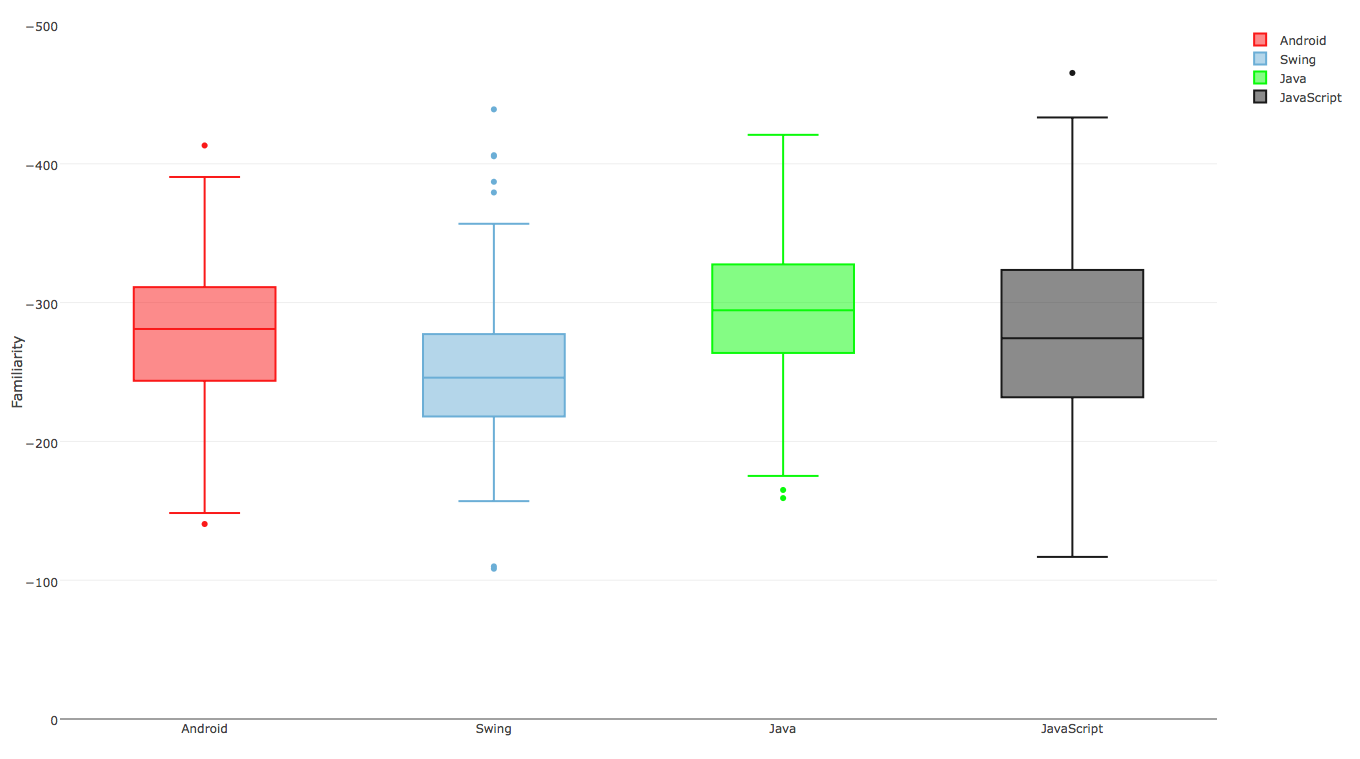
\includegraphics[width=\textwidth]{code100}
			\caption{Code LM trained with 100 documents}
			\label{code100}
			\end{figure}		
\newpage

With a training set of 1000 Android documents we start observing some changes, as we can see in Fig \ref{code1000}, Android testing documents are more familiar than Java and significantly more familiar than JavaScript.

\begin{figure}[H]
			\centering
			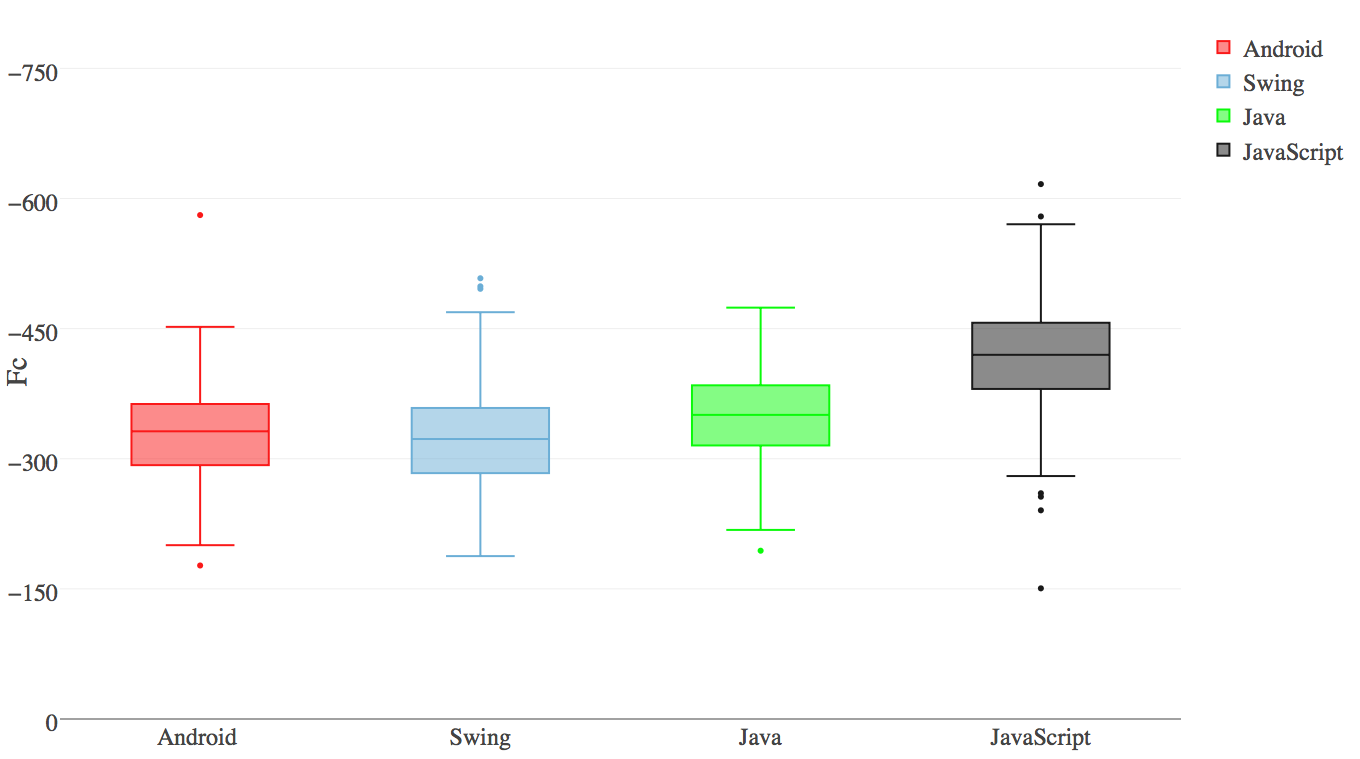
\includegraphics[width=\textwidth]{code1000}
			\caption{Code LM trained with 1000 documents}
			\label{code1000}
			\end{figure}

 

\begin{figure}[H]
			\centering
			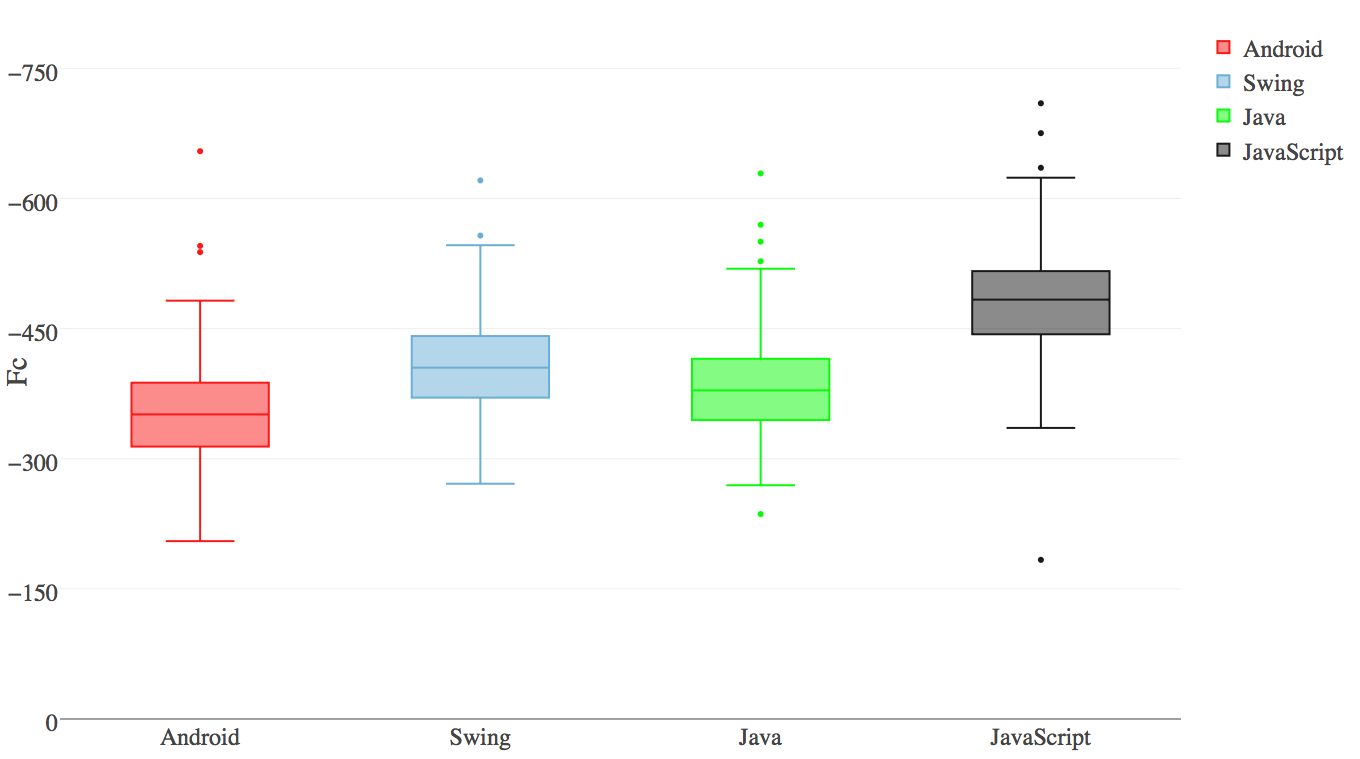
\includegraphics[width=\textwidth]{code10000}
			\caption{Code LM trained with 10000 documents}
			\label{code10000}
			\end{figure}		
In Fig \ref{code10000}, we can see that with a training set of 10,000 documents, Android is estimated as the most familiar, followed by Java; then Swing and JavaScript are clearly less familiar.

This result reflects our expectation, where Android is expected to be the most familiar, since the training set contains only Android documents, and as Android is implemented in Java we expected that Java should be more familiar than JavaScript and Swing. We have to mention that the familiarity result is logarithmic, therefore a small difference between the boxes position has to be interpreted as a big difference between the familiarity of the boxes.  

\begin{figure}[H]
			\centering
			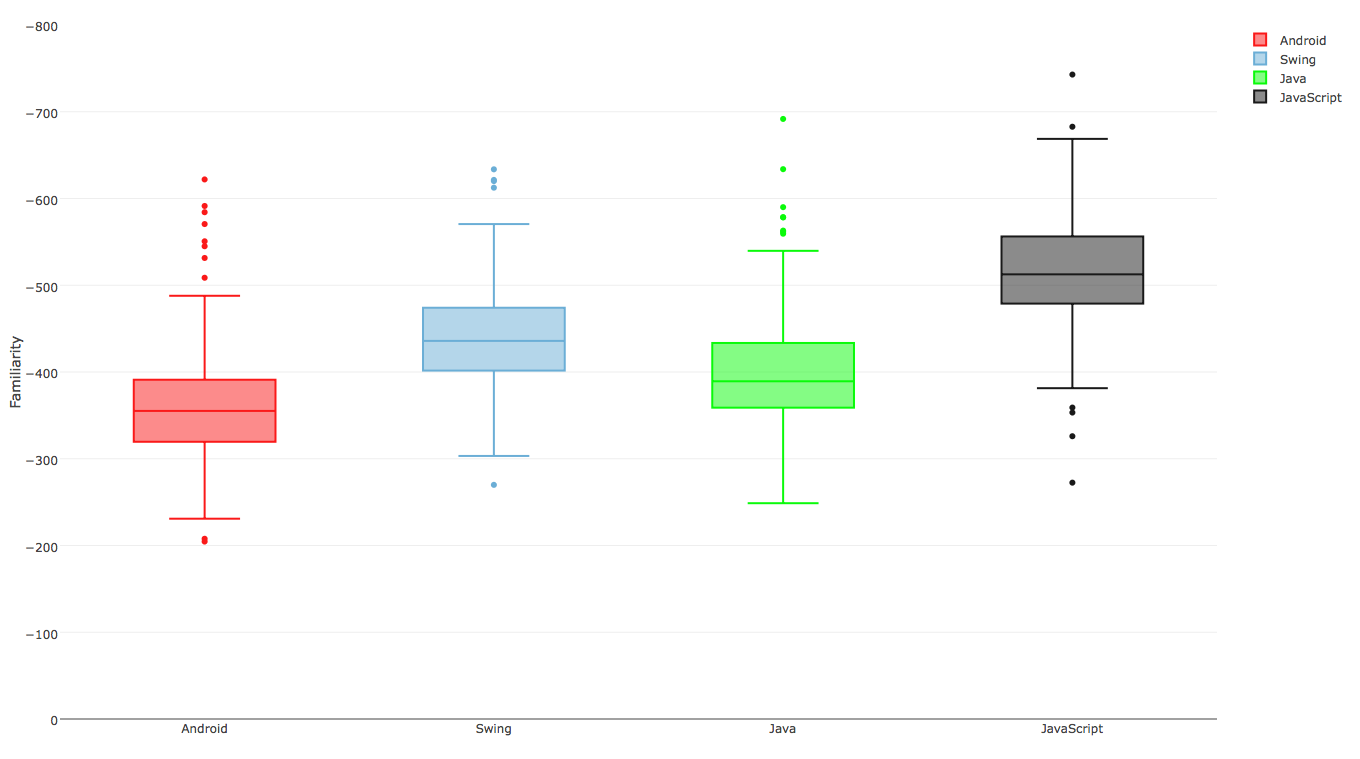
\includegraphics[width=\textwidth]{code100000}
			\caption{Code LM trained with 100000 documents}
			\label{code100000}
\end{figure}	

 We also train the code LM with a set of 100,000 Android documents and as we can see in Fig \ref{code100000}, the result is similar to Fig \ref{code10000} (where the training set contains 10,000 documents).

These results infer that a LM can capture the familiarity of code, and bigger is the training set better is the performance.


\subsection{Text LM Results}

 As we did for the Code LM, we train the text LM with 10, 100, 1000, 10,000 and 100,000 Android documents, and for each training set we estimate the familiarity of the testing set.\newpage
	
In Fig \ref{text10} and Fig \ref{text100}, we can see that Android documents are not the most familiar documents, and the reason is the small size of the training set (10 in Fig \ref{text10} and 100 in Fig \ref{text100}).

\begin{figure}[H]
			\centering
			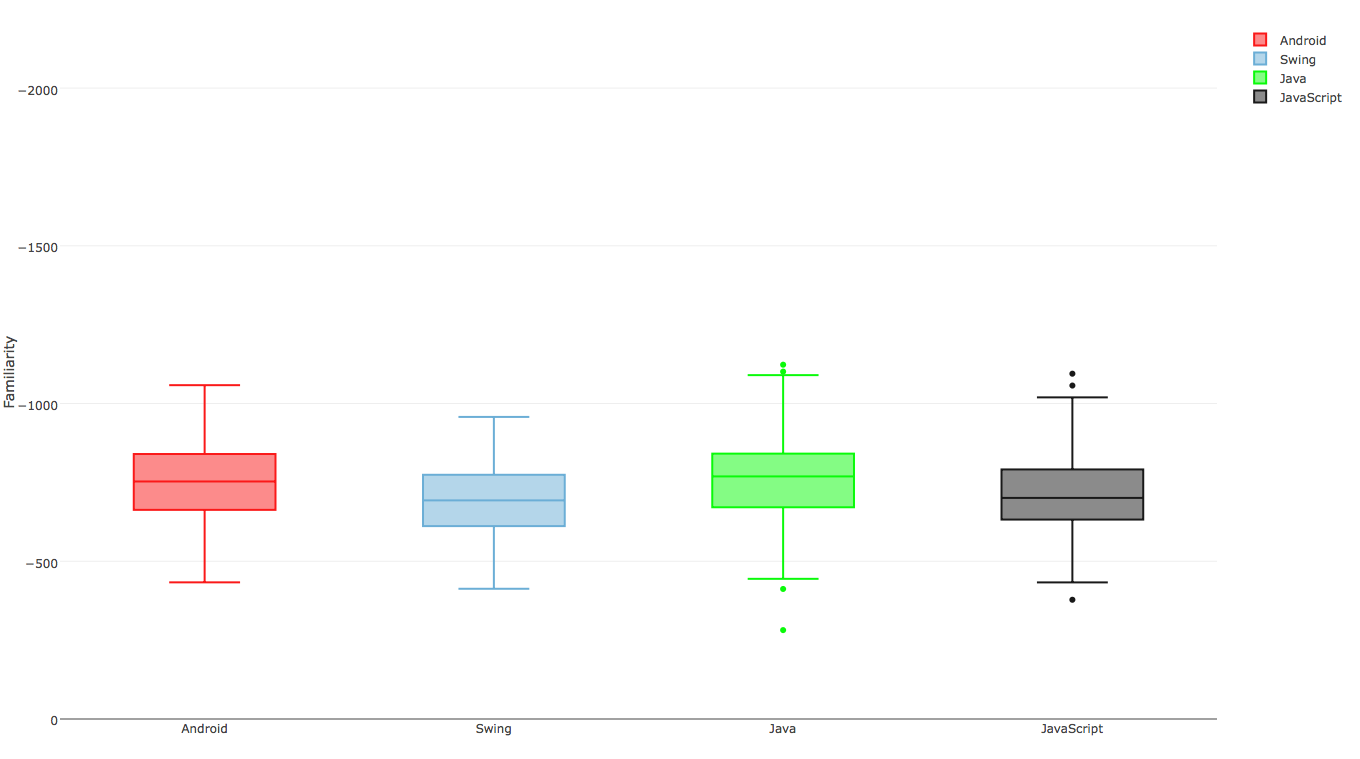
\includegraphics[width=\textwidth]{text10}
			\caption{Code LM trained with 10 documents}
			\label{text10}
\end{figure}

\begin{figure}[H]
			\centering
			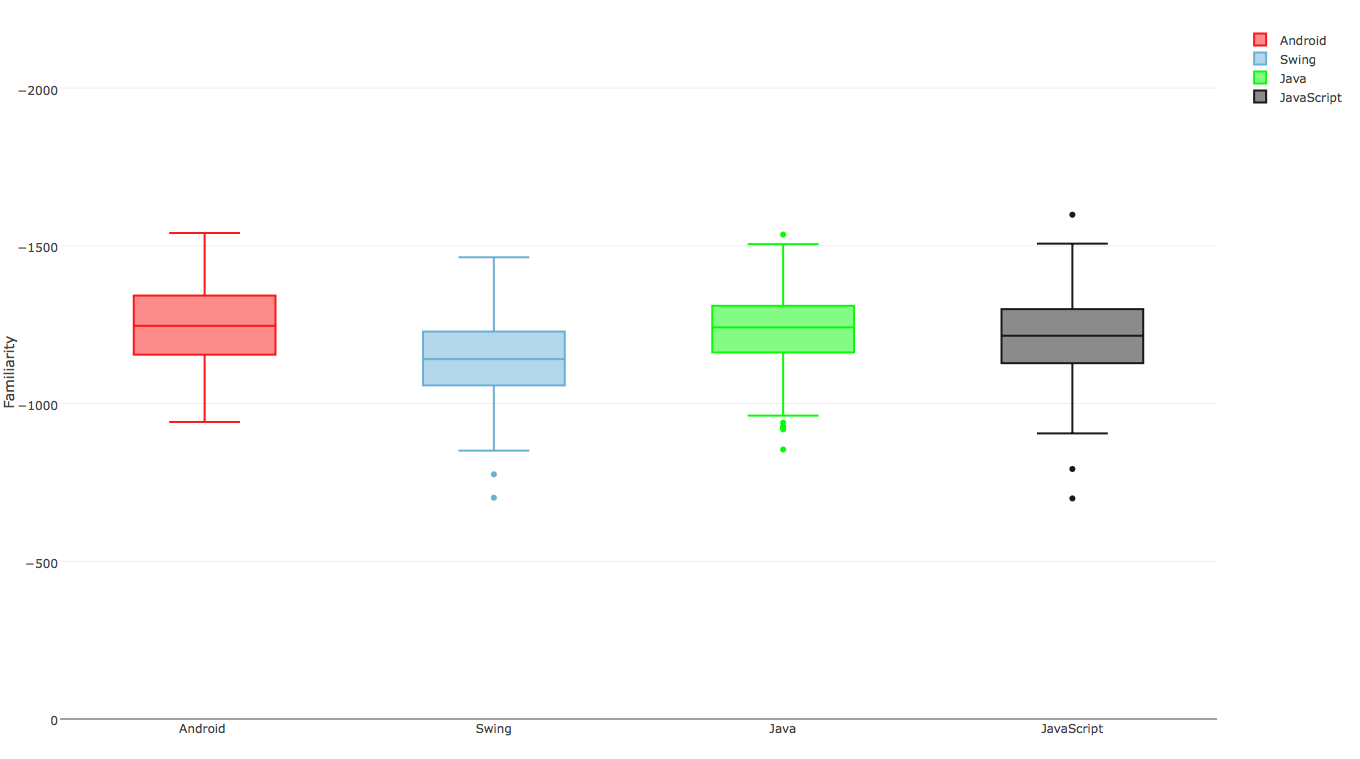
\includegraphics[width=\textwidth]{text100}
			\caption{Code LM trained with 100 documents}
			\label{text100}
\end{figure}

In Fig \ref{text1000}, we can see that when we train the text LM with 1000 Android documents, Android is estimated as more familiar than Java and JavaScript, and in Figure \ref{text10000} we train the code LM with 10,000 documents which estimate Android as the most familiar.

\begin{figure}[H]
			\centering
			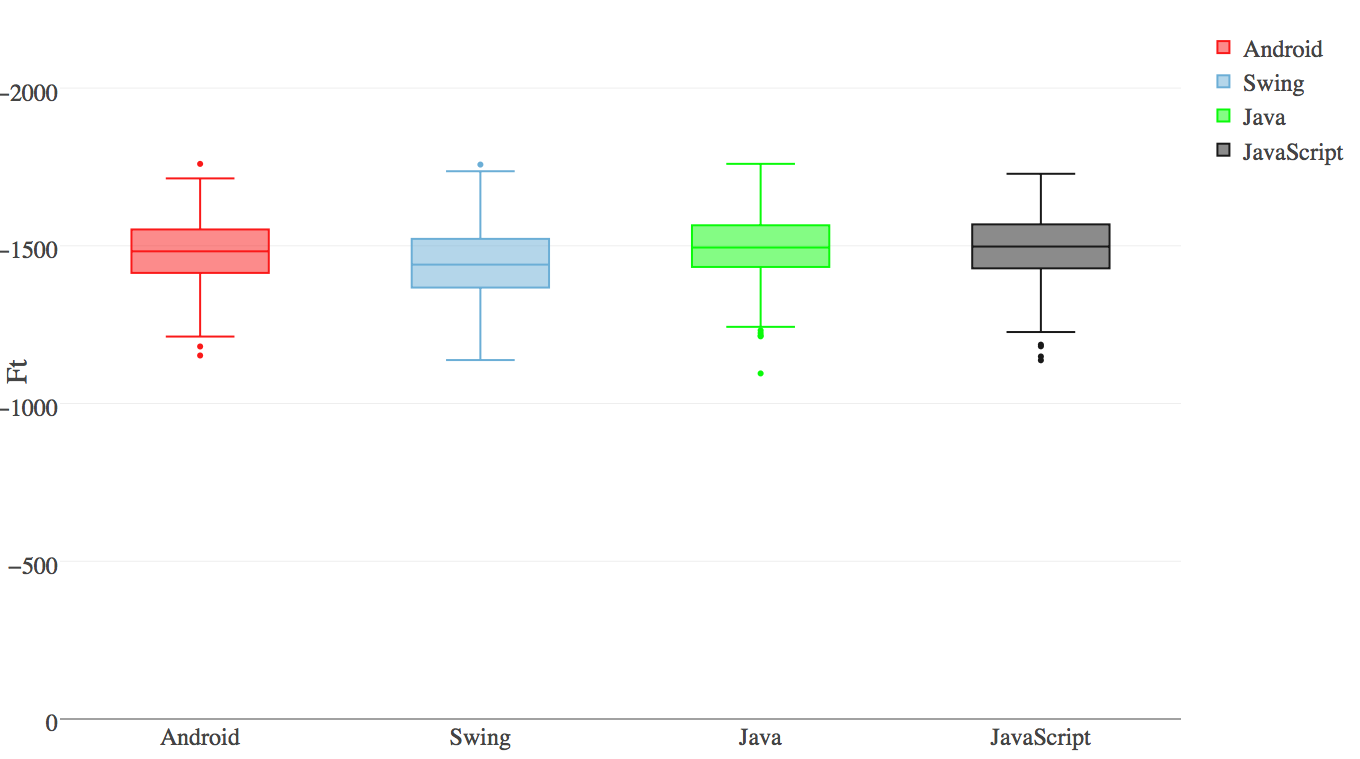
\includegraphics[width=\textwidth]{text1000}
			\caption{Code LM trained with 1000 documents}
			\label{text1000}
\end{figure}

\begin{figure}[H]
			\centering
			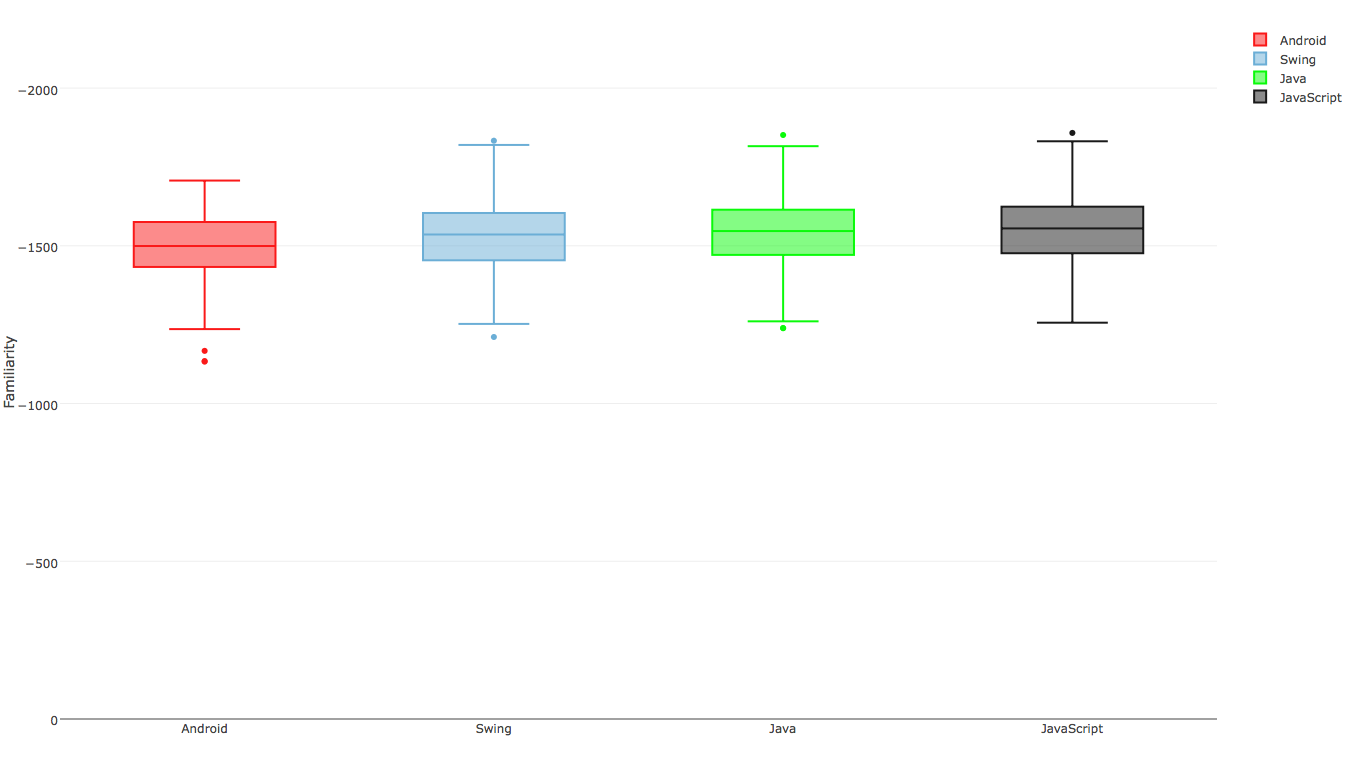
\includegraphics[width=\textwidth]{text10000}
			\caption{Code LM trained with 10000 documents}
			\label{text10000}
\end{figure}

We get the expected result when we train the text LM with as set of 100000 documents. In Fig \ref{text100000}, we can see that Android is the most familiar and then Java which is more familiar than JavaScript and Swing.
\begin{figure}[H]
			\centering
			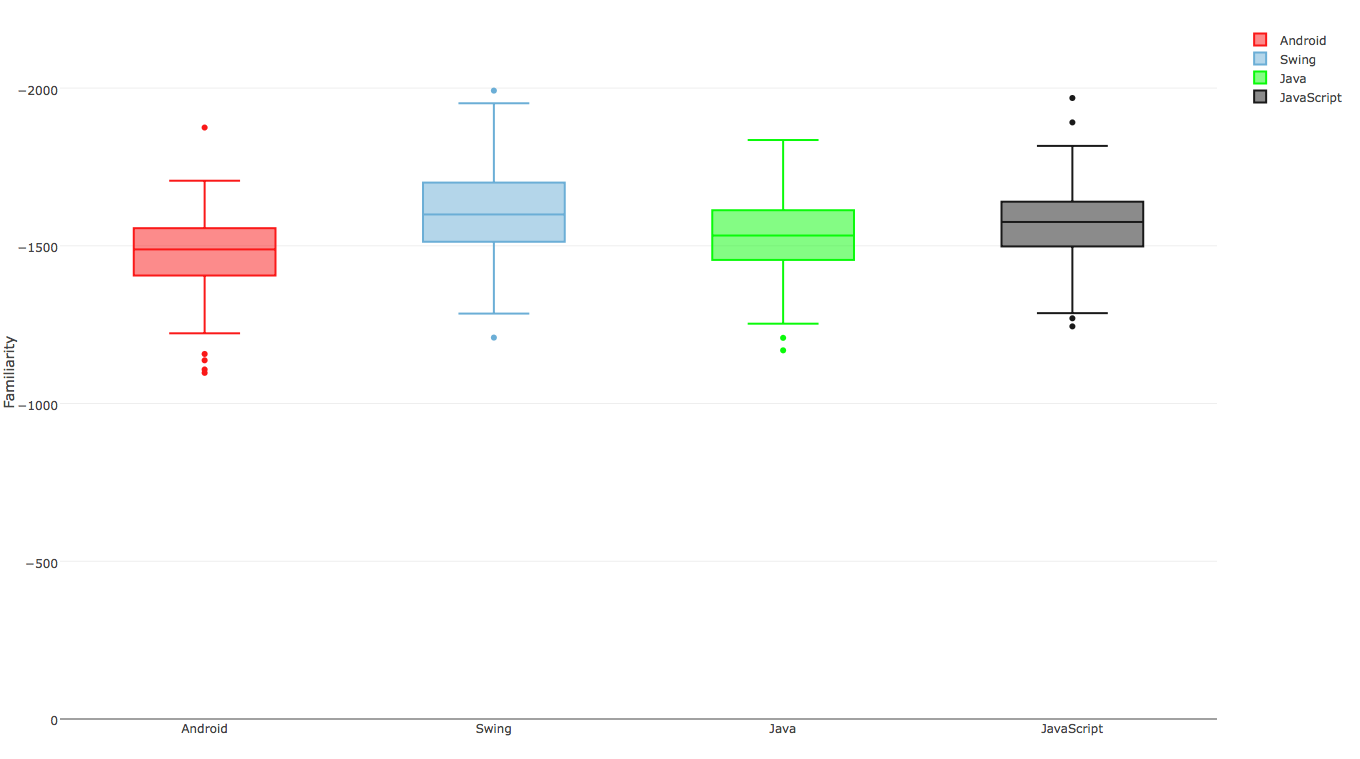
\includegraphics[width=\textwidth]{text100000}
			\caption{Code LM trained with 100000 documents}
			\label{text100000}
\end{figure}
These results infer that the LM can capture the familiarity of text, but to get a better performance we need to train the LM with a large set of documents.

\section{Comprehension Effort Estimation Results}

To evaluate our comprehension effort estimation, we ask two developers to read 4 introduction tutorials to Android, and one Android-Camera API tutorial and one Android-Bluetooth API tutorial, and as described in the Chapter 4.1, we ask them to score the comprehension effort of 6 documents on a scale of 0 to 5, where a higher score means a higher effort. In the meanwhile, we train the LMs and we estimate the comprehension effort that we compare with their score. 



\begin {table}[H]
	\begin{center}
    \begin{tabular}{| l | l | l | l | l | l | l | l |}
    \hline
\textbf{Tutorial}	&  \textbf{$F_{c}$}	& \textbf{$F_{t}$}	& \textbf{$R_c$}	& \textbf{$R_t$}	& \textbf{Effort}	& \textbf{ Dev 1}&  \textbf{Dev 2}\\ \hline
Bluetooth   & -2694.64	& -377.42	& 0.1979 	& 0.5439	& 1166.6	& 1	& 1\\ \hline
Camera		& -2794.77	& -309.74	& 0.1570	& 0.4713	& 1259.8	& 2	& 2\\ \hline
AsyncTask	& -3446.07	& -265.87	& 0.2537	& 0.5301	& 1348.2	& 3	& 3\\ \hline
Database	& -3491.46	& -336.06	& 0.2472	& 0.6235	& 1377.4	& 4	& 3\\ \hline
Cordova-1	& -4539.99	& -313.44	& 0.3377	& 0.4952	& 1582.5	& 4	& 1\\ \hline
Cordova-2	& -4429.52	& -273.63	& 0.1579	& 0.4173	& 1944.5	& 2	& 1\\ \hline
   \end{tabular}
	\end{center}
	\caption{Comprehension effort evaluation} \label{tab:comprehension-effort} 
	\end{table}

In the Table \ref{tab:comprehension-effort} for each tutorial we show our estimation effort, that we derive from the code and text readability and familiarity.
\[\text{Comprehension Effort = }\frac{(r_{c}\times f_{c}) + (r_{t} \times f_{t})}{2} \]

The table contains also the developers scores (Score 1, Score 2). As we can see, our approach estimates \emph{Bluetooth} and \emph{Camera} tutorials as the documents that require less effort to be comprehended, and both developers gave them a low score (1 and 2), we also estimate that \emph{AsyncTask} and \emph{Database} require more effort, and also both developers gave them a higher score (3 and 4).

We estimate \emph{Cordova-1} and \emph{Cordova-2} to require the highest effort. The first developer gave them 4 and 2 which still a high score, but the second developer gave them 1, which is a low score. We asked the developer if he can justify the low score that he gave to the \emph{Corodova}s documents, and he points out that JavaScript is the programing language that he knows best. Therefore, he is familiar with JavaScript, and Cordova is implemented with JavaScript, which justify the low score.


The evaluation results suggest that our approach is promising in estimating the comprehension effort of developers. 


\section{Summary}
To evaluate our familiarity estimation approach, we run an experiment where we evaluate the LM efficiency in estimating the familiarity of a given document. In this experiment we tried different training sets sizes, and the results showed that 10 or 100 training documents are not enough to build a LM able to capture the familiarity. The LM needs larger set to perform well. With a training set of 10,000 documents we got a very good performance. Lager is the training set better is the LM performance.

To evaluate the comprehension effort estimation approach, we ask two developers to read a set of tutorials and then to score a set of StackOverflow discussions and we compare their score with our precomputed score. The results indicate that our score match with the developers score, therefore we believe that our approach is promising in estimating the comprehension effort.


\chapter{Threats to Validity}
\section{Experiment-1}

Two potential threats to validity concern the training and testing sets in Experiment-1.
The experiment is based on training LMs on Android discussions and evaluating the familiarity of different testing sets (Android, Java, Swing, JavaScript). The experiment considers only Android framework to show that LMs are efficient in estimating Android familiarity, but we didn't run other studies to evaluate our approach on different frameworks. To generalize our approach we need to evaluate other frameworks or even other programming languages. We will investigate this further in future research.

The testing and training sets are StackOverflow discussions, where documents contain code snippets and text. In this experiment, the code LM is trained on small and some times incomplete code. If we run this experiment in a different context as any system where the code is complete and much bigger than Stack Overflow discussions, we might have different performance in estimating the familiarity.

\section{Experiment-2}
In Experiment-2, the main threats are related to the data set size. In this study, we asked two developers who have no experience with Android framework to read a set of 6 Android tutorials (training set) and to score the comprehension effort of a set of Stack Overflow discussions (testing set). To compare the developers' scores with our estimation we trained the LMs with the same training set. But as we mentioned in Chapter 5.1 the LM requires a large training set to perform well, and 6 tutorials are too few. Therefore, we trained the code LM  with a large set of Gist code snippets that have the same subject as the tutorials. This procedure can introduce some inconsistency since the training set that we gave to LMs is different form the one that we gave to the developers.

In this experiment, we compare our comprehension effort estimation with two developers scores. In order to generalize our approach, we need to run our experiment on a bigger sample. Furthermore, we couldn't run any statistical analysis as calculating the precision and accuracy of our approach because the sample size is too small, but this experiment is a starting point which suggests that our approach is promising in estimating the comprehension effort. We will investigate this further in future research.




\chapter{Conclusion}

In this thesis, we have presented and evaluated the first approach in the literature able to assess documents by comprehension effort. The comprehension effort is based on the readability and the familiarity of the document. We have conducted a study over 100,000 Stack Overflow documents aimed to evaluate the language model efficiency to estimate the familiarity of a given document. The achieved results have shown that language model is able to estimate the familiarity and we noticed that its performance is tightly related to the training set size. The best results have been achieved with a training set size $\ge$ 10,000 Stack Overflow documents.

In addition, we have conducted a study to evaluate our approach in estimating the comprehension effort. The sample size was not big enough to generalize the findings of your study, but the achieved results suggest that our approach is promising in estimating the comprehension effort.

In the future studies aimed at replicating our work, we advise running the familiarity evaluation experiment on a different framework or programing language. For example, to train a LM on Java and to evaluate its efficiency in predicting the familiarity of Java and a C++ sets, where these two programing languages have a similar syntax. 


We also advise running the comprehension effort evaluation experiment on a large sample in order to generalize our estimating approach. Moreover, we encourage future works to explore the alternative comprehension effort estimating formula that we proposed in Chapter 3.4 :
 \[\text{Comprehension Effort = }\frac{(r_{c}\times f_{c}) + (r_{t} \times f_{t})}{r_c+r_t} \] 
where \emph{familiarity} has a higher weight, and to compare its precision and accuracy with the formula that we used in our experiment:

 \[\text{Comprehension Effort = }\frac{(r_{c}\times f_{c}) + (r_{t} \times f_{t})}{2} \]
 
where the \emph{readability} and the \emph{familiarity} have the same weight.


We also suggest the RSSE as LIBRA to take advantage of our comprehension effort metric to improve their suggestions.

Finally, it is important to note that the comprehension effort metric described in this thesis is not intended as the final model where only the readability and familiarity of a document determine the 
required human effort to comprehend it. Other metrics, (e.g., cyclomatic complexity) can be explored and added to readability and familiarity metrics to compute the comprehension effort.





% \chapter[Short title]{A chapter title which will run over two lines --- it's for
%   testing purpose}


% \textbf{Theorem 1 (Residue Theorem).}
% Let $f$ be analytic in the region $G$ except for the isolated singularities $a_1,a_2,\ldots,a_m$. If $\gamma$ is a closed rectifiable curve in $G$ which does not pass through any of the points $a_k$ and if $\gamma\approx 0$ in $G$ then
% \[
% \frac{1}{2\pi i}\int_\gamma f = \sum_{k=1}^m n(\gamma;a_k) \text{Res}(f;a_k).
% \]
% \textbf{Theorem 2 (Maximum Modulus).}
% \emph{Let $G$ be a bounded open set in $\mathbb{C}$ and suppose that $f$ is a continuous function on $G^-$ which is analytic in $G$. Then}
% \[
% \max\{|f(z)|:z\in G^-\}=\max \{|f(z)|:z\in \partial G \}.
% \]

% \section[third]{A very very long section, titled ``The third section'', with
%   a rather  short text alternative (third)}



\nocite{*}

\appendix %optional, use only if you have an appendix



\backmatter

%\chapter{Glossary} %optional

%\bibliographystyle{alpha}
%\bibliographystyle{dcu}
\bibliographystyle{plainnat}
\bibliography{biblio}

%\cleardoublepage
%\theindex %optional, use only if you have an index, must use
	  %\makeindex in the preamble


\end{document}
